\subsection{Application to the Brauer Group}

In this subsection, K is a field, and L is a Galois algebra over K with action \(\lambda: G \to \operatorname{Aut}_{K}(L)\) . We denote the degree of L over K by n.~We have \(n = \operatorname{Card}(G)\) .

THEOREM 3. --- Let \(\mathcal{E} = (\Gamma, \iota, \pi)\) be a \(\tau\) -extension of G by L*. The algebra \(\mathbf{A}[\mathcal{E}; \mathrm{L}]\) is central simple and of degree \(n^2\) over K. Moreover, the canonical homomorphism \(u\) from L to \(\mathbf{A}[\mathcal{E}; \mathrm{L}]\) is an isomorphism from L to a maximal commutative subalgebra of \(\mathbf{A}[\mathcal{E}; \mathrm{L}]\) .

Lemma 12. --- a) There does not exist any ideal of L, other than \(\{0\}\) and L that is invariant under G.

\begin{enumerate}
\def\labelenumi{\alph{enumi})}
\setcounter{enumi}{1}
\tightlist
\item
  Let g be an element of G distinct from the identity element, and let \(\mathfrak{a}_{g}\) be the ideal of L generated by the elements of the form \(x - \lambda(g)x\) , where x runs through L. We have \(\mathfrak{a}_{g} = L\) .
\end{enumerate}

Let \(\mathscr{S}\) be the set of maximal ideals of L; for any subset S of \(\mathscr{S}\), set \(\mathfrak{a}(S) = \bigcap_{\mathfrak{m} \in S} \mathfrak{m}\) . Since the ring L is commutative and semisimple (VIII, p.~310, Remark 6), the map \(W \mapsto \mathfrak{a}(W)\) is a bijection from the set of subsets of \(\mathscr{S}\) to the set of ideals of L (VIII, p.~142, Proposition 9). The ideal \(\mathfrak{a}(S)\) is invariant under G if and only if S is. Since G acts transitively on \(\mathscr{S}\) (VIII, p.~308, Theorem 2, vi)), the only subsets of \(\mathscr{S}\) invariant under G are \(\varnothing\) and \(\mathscr{S}\). Since \(\mathfrak{a}(\varnothing) = L\) and \(\mathfrak{a}(\mathscr{S}) = \{0\}\) , we have proved assertion a).

Let us prove b) by contradiction; suppose that we have \(\mathfrak{a}_g\neq \mathrm{L}\) . Let \(\mathfrak{m}\) be a maximal ideal of L containing \(\mathfrak{a}_g\) . We then have \(\lambda (g)x\equiv x\bmod \mathfrak{m}\) for every x in L. In particular, m is invariant under g, and \(\lambda(g)\) is induced by the identity on the field L/m. By property (vi) in Theorem 2 of VIII, p.~308, the element g of \(G_{m}\) is trivial, which contradicts the assumption of b).

Let us now prove Theorem 3. The vector space \(\mathbf{A}[\mathcal{E};\mathrm{L}]\) has finite dimension \(\operatorname{Card}(\mathrm{G})[\mathrm{L}:\mathrm{K}] = n^2\) over \(\mathrm{K}\) , by VIII, p.~316 and the assumed equality \(\operatorname{Card}(\mathrm{G}) = [\mathrm{L}:\mathrm{K}] = n\) .

Let \(\mathfrak{a}\) be a nonzero two-sided ideal of the algebra \(\mathbf{A}[\mathcal{E};\mathrm{L}]\) . We use the notation of VIII, p.~316. Every element \(a\) of \(\mathbf{A}[\mathcal{E};\mathrm{L}]\) can be written uniquely as \(a = \sum_{g\in \mathrm{G}}a_g\varepsilon_g\) with \(a_g\in \mathrm{L}\) for every \(g\in \mathrm{G}\) ; we denote by \(\Phi (a)\) the set of elements \(g\) of \(\mathrm{G}\) such that \(a_g\neq 0\) . By formula (32) of VIII, p.~316, we have the relation

\[
\varepsilon_ {g} \varepsilon_ {g ^ {\prime}} = c _ {\sigma} (g, g ^ {\prime}) \varepsilon_ {g g ^ {\prime}}\tag{38}
\]

for all \(g, g' \in \mathrm{G}\) and consequently

\[
\Phi (a \varepsilon_ {g}) = \Phi (a). g\tag{39}
\]

for every \(g\in \mathbf{G}\) and \(a\in \mathbf{A}[\mathcal{E};\mathrm{L}]\) .

Let \(a\) be a nonzero element of \(\mathfrak{a}\) for which \(\Phi(a)\) is minimal for the inclusion; by formula (39), if necessary replacing \(a\) with an element of the form \(a\varepsilon_{g^{-1}}\) with \(g\in\Phi(a)\) , we may assume that we have \(e\in\Phi(a)\) . Let \(s\) be an element of \(\Phi(a)\) distinct from \(e\) . By Lemma 12, b), there exists an element \(x\) of L such that \(a_s(x-\lambda(s)\cdot x)\neq0\) . But we have the relation

\[
x a - a x = \sum_ {g} a _ {g} (x - \lambda (g) \cdot x) \varepsilon_ {g},\tag{40}
\]

where the sum is taken over the elements g of \(\Phi(a)\) distinct from e. Because of the minimality of \(\Phi(a)\) , we then have xa - ax = 0, but this contradicts the assumption on x. We have, therefore, proved by contradiction that \(\Phi(a)\) contains only the identity element e of G, so we have \(a \in L\) .

Hence \(L \cap a\) is an ideal of L not reduced to \(\{0\}\) . Moreover, for every x in L, we have \(\varepsilon_{g}x\varepsilon_{g}^{-1} = \lambda(g) \cdot x\) , so \(L \cap a\) is invariant under G. By Lemma 12, we therefore have \(L \cap a = L\) , that is, \(L \subset a\) . Since L contains the identity element of \(A[E;L]\) , we have \(a = A[E;L]\) .

Since the algebra \(A[E;L]\) has nonzero finite dimension over K and its only two-sided ideals are \(\{0\}\) and \(A[E;L]\) , it is simple.

Let us prove that every element \(a\) of \(\mathbf{A}[\mathcal{E};\mathrm{L}]\) that commutes with L belongs to L. We write \(a\) as \(\sum_{g\in \mathrm{G}}a_g\varepsilon_g\) with coefficients \(a_{g}\) in L. For every \(x\) in L, we have \(xa - ax = 0\) , and relation (40) shows that we have

\[
a _ {g} (x - \lambda (g) \cdot x) = 0\tag{41}
\]

for every \(g \in \mathrm{G}\) and \(x \in \mathrm{L}\) . By Lemma 12, we therefore have \(a_g = 0\) for \(g \neq e\) ; consequently, \(a \in \mathrm{L}\) .

Let us, finally, determine the center of \(\mathbf{A}[\mathcal{E};\mathrm{L}]\) . If \(z\) belongs to the center, then it commutes with \(\mathrm{L}\) , so belongs to \(\mathrm{L}\) . But we then have

\[
0 = \varepsilon_ {g} z - z \varepsilon_ {g} = (\lambda (g) \cdot z - z) \varepsilon_ {g}
\]

for every g of G. Hence z is invariant under the automorphism group \(\lambda(\mathrm{G})\) of L. We therefore have \(z \in K\) by assumption.

THEOREM 4. --- Let A be a central simple algebra of finite degree over K, and let L be a maximal commutative subalgebra of A. Then there exists a \(\tau\) -extension \(\mathcal{E}\) of G by \(\mathrm{L}^*\) such that A is isomorphic to \(\mathbf{A}[\mathcal{E};\mathrm{L}]\) .

Without loss of generality, we may assume that L is a maximal commutative subalgebra of A. Let \(\Gamma\) be the multiplicative group consisting of the invertible elements \(\gamma\) of A such that there exists a g in G with

\[
\gamma x \gamma^ {- 1} = \lambda (g). x\tag{42}
\]

for every element x of L. If \(\gamma \in \Gamma\) is given, then the element g satisfying this relation is unique; we denote it by \(\pi(\gamma)\) . It is immediate that \(\pi\) is a homomorphism from \(\Gamma\) to G and that its kernel is equal to \(L^{*}\) . The surjectivity of \(\pi\) follows from the Skolem--Noether theorem (VIII, p.~263, Corollary).

If we denote the canonical injection of \(L^{*}\) into \(\Gamma\) by \(\iota\) , then it follows from the constructions that \(\mathcal{E} = (\Gamma, \iota, \pi)\) is a \(\tau\) -extension of G by \(L^{*}\) . Let

\[
u: \mathrm{L} \to \mathbf {A} [ \mathcal {E}; \mathrm{L} ] \quad \text { and } \quad v: \Gamma \to \mathbf {A} [ \mathcal {E}; \mathrm{L} ]
\]

be the canonical homomorphisms. By the universal property of \(\mathbf{A}[\mathcal{E};\mathrm{L}]\) (VIII, p.~315, Proposition 12), there exists a unique algebra homomorphism \(f:\mathbf{A}[\mathcal{E};\mathrm{L}]\to \mathrm{A}\) such that \(f\circ u(x) = x\) and \(f\circ v(\gamma) = \gamma\) for \(x\in \mathrm{L}\) and \(\gamma \in \Gamma\) . Since the algebra \(\mathbf{A}[\mathcal{E};\mathrm{L}]\) is simple, the homomorphism \(f\) is injective. Now, the algebra \(\mathbf{A}[\mathcal{E};\mathrm{L}]\) has degree \(n^2\) over \(\mathbf{K}\) and so does \(\mathrm{A}\) because \(\mathrm{L}\) is a maximal commutative semisimple subalgebra of \(\mathrm{A}\) and we have \(n = [\mathrm{L}:\mathrm{K}]\) (VIII, p.~262, Proposition 3, (ii)). Hence \(f\) is bijective.

DEFINITION 2. --- Let \(\mathscr{S}\) be the set of maximal ideals of L. We define

\[
\operatorname{Br} (\mathrm{L} / \mathrm{K}) = \bigcap_ {\mathfrak {m} \in \mathscr {S}} \operatorname{Ker} (r _ {(\mathrm{L} / \mathfrak {m}) / \mathrm{K}}),
\]

where \(r_{(L/\mathfrak{m})/K} : \mathrm{Br}(K) \to \mathrm{Br}(L/\mathfrak{m})\) is the extension of scalars homomorphism (VIII, p.~281).

THEOREM 5. --- There exists a group isomorphism

\[
\Psi : \mathrm{Ex} _ {\tau} (\mathrm{G}, \mathrm{L} ^ {*}) \longrightarrow \mathrm{Br} (\mathrm{L} / \mathrm{K})
\]

that sends the class of a \(\tau\) -extension \(\mathcal{E}\) of G by \(\mathrm{L}^*\) to the class in \(\mathrm{Br}(\mathrm{L} / \mathrm{K})\) of the algebra \(\mathbf{A}[\mathcal{E};\mathrm{L}]\) .

To define \(\Psi\) and verify that it is a bijection, we must establish the following points:

\begin{enumerate}
\def\labelenumi{\alph{enumi})}
\item
  If \(\mathcal{E}\) and \(\mathcal{E}'\) are isomorphic \(\tau\) -extensions of \(G\) by \(L^*\) , then the algebras \(\mathbf{A}[\mathcal{E}; L]\) and \(\mathbf{A}[\mathcal{E}'; L]\) are isomorphic.
\item
  Conversely, if the algebras \(\mathbf{A}[\mathcal{E};\mathrm{L}]\) and \(\mathbf{A}[\mathcal{E}';\mathrm{L}]\) are isomorphic, then the \(\tau\) -extensions \(\mathcal{E}\) and \(\mathcal{E}'\) of \(\mathrm{G}\) by \(\mathrm{L}^*\) are isomorphic.
\item
  In every class in \(\mathrm{Br(L / K)}\) , there is an algebra \(E\) containing \(L\) as a maximal commutative subalgebra.
\item
  If \(\mathrm{E}\) is a central simple algebra of finite degree over \(\mathrm{K}\) containing \(\mathrm{L}\) as a maximal commutative subalgebra, then there exists a \(\tau\) -extension \(\mathcal{E}\) of \(\mathrm{G}\) by \(\mathrm{L}^*\) such that \(\mathrm{E}\) is isomorphic to \(\mathbf{A}[\mathcal{E};\mathrm{L}]\) .
\end{enumerate}

Assertion a) follows from the construction of the cross product; b) follows from VIII, p.~263, Corollary. Assertion c) follows from Proposition 5 of VIII, p.~281, and d) is simply Theorem 4 above.

It remains to verify that \(\Psi\) is a group homomorphism; for this, it suffices to prove that if \(\mathcal{E}_1 = (\Gamma_1,\iota_1,\pi_1)\) and \(\mathcal{E}_2 = (\Gamma_2,\iota_2,\pi_2)\) are \(\tau\) -extensions, then the algebra \(\mathbf{A}[\mathcal{E}_1\mathcal{E}_2;\mathrm{L}]\) is equivalent to the algebra \(\mathbf{A}[\mathcal{E}_1;\mathrm{L}]\otimes \mathbf{A}[\mathcal{E}_2;\mathrm{L}]\) . We denote the product extension \(\mathcal{E}_1\mathcal{E}_2\) by \(\mathcal{E} = (\Gamma ,\iota ,\pi)\) . The group \(\Gamma\) is isomorphic to the cokernel of the homomorphism \(\rho\) from \(\mathrm{L}^*\) to the fiber product \(\Gamma_1\times_{\mathrm{G}}\Gamma_2\) that sends \(\mu\) to \((\iota_1(\mu),\iota_2(\mu)^{-1})\) . For \(i\in \{1,2\}\) , write \(\mathrm{A}_i = \mathbf{A}[\mathcal{E}_i;\mathrm{L}]\) . Let \(u_{i}:\mathrm{L}\to \mathrm{A}_{i}\) and \(v_{i}:\Gamma_{i}\rightarrow \mathrm{A}_{i}^{*}\) be the canonical homomorphisms. We identify L with its images by the homomorphisms \(u_{i}\) , which make L into maximal commutative subalgebras of the \(\mathrm{A}_i\) . We denote by \(\mathrm{V}_i\) the L-vector space defined by left multiplication in \(\mathrm{A}_i\) . The ring \(\mathrm{L}\otimes_{\mathrm{K}}\mathrm{A}_i^{\circ}\) acts on \(\mathrm{V}_i\) . Since it is simple and has dimension \(n^2\) over L, we obtain an isomorphism from \(\mathrm{L}\otimes_{\mathrm{K}}\mathrm{A}_i^{\circ}\) to \(\operatorname {End}_{\mathrm{L}}(\mathrm{V}_{i})\) . Hence the ring \(\mathrm{L}\otimes_{\mathrm{K}}\mathrm{A}_1^{\circ}\otimes_{\mathrm{K}}\mathrm{A}_2^{\circ}\) , which we can identify with \((\mathrm{L}\otimes_{\mathrm{K}}\mathrm{A}_1^{\circ})\otimes_{\mathrm{L}}(\mathrm{L}\otimes_{\mathrm{K}}\mathrm{A}_2^{\circ})\) , is isomorphic to \(\operatorname {End}_{\mathrm{L}}(\mathrm{V}_{1}\otimes_{\mathrm{L}}\mathrm{V}_{2})\) . Set \(\mathrm{C} = \operatorname {End}_{\mathrm{A}_1^{\circ}\otimes_{\mathrm{K}}\mathrm{A}_2^{\circ}}(\mathrm{V}_1\otimes_\mathrm{L}\mathrm{V}_2)\) . By Lemma 3 of VIII, p.~282, the ring C is similar to \(\mathrm{A}_1\otimes_{\mathrm{K}}\mathrm{A}_2\) , and \(\mathrm{L}\otimes 1\otimes 1\) is a maximal commutative subalgebra of C. For every pair \((\gamma_{1},\gamma_{2})\in \Gamma_{1}\times \Gamma_{2}\) satisfying \(\pi_1(\gamma_1) = \pi_2(\gamma_2)\) , we denote by \(w(\gamma_1,\gamma_2)\)

the unique \(\lambda (\pi_1(\gamma_1))\) -semilinear (II, §1, No.~13, p.~223) endomorphism such that

\[
w (\gamma_ {1}, \gamma_ {2}) (x _ {1} \otimes x _ {2}) = v _ {1} (\gamma_ {1}) x _ {1} \otimes v _ {2} (\gamma_ {2}) x _ {2}
\]

for \(x_{1} \in V_{1}\) and \(x_{2} \in V_{2}\) . We have \(w(\gamma_{1}, \gamma_{2}) \in \mathrm{C}^{*}\) , and w is a group homomorphism from the fiber product \(\Gamma_{1} \times_{G} \Gamma_{2}\) to \(C^{*}\) . This homomorphism is trivial on the image of \(\rho\) and induces a homomorphism v from \(\Gamma\) to \(C^{*}\) . Denote by \(u : L \to C\) the morphism given by \(u : \ell \mapsto \ell \otimes 1 \otimes 1\) . We can verify the relations

\[
u (\alpha) = v (\iota (\alpha)) \quad \text { and } \quad u (^ {\gamma} \beta) = v (\gamma) u (\beta) v (\gamma) ^ {- 1}
\]

for \(\alpha \in \mathrm{L}^*\) , \(\beta \in \mathrm{L}\) , and \(\gamma \in \Gamma\) . Proposition 12 of VIII, p.~315 gives a homomorphism \(f\) from the algebra \(\mathbf{A}[\mathcal{E};\mathrm{L}]\) to \(\mathrm{C}\) . Since the algebra \(\mathbf{A}[\mathcal{E};\mathrm{L}]\) is simple, the homomorphism \(f\) is injective. The algebras \(\mathrm{C}\) and \(\mathbf{A}[\mathcal{E};\mathrm{L}]\) have the same dimension over \(\mathrm{K}\) , so \(f\) is an isomorphism.

Remarks. --- 1) If L is an étale algebra over K and G is the automorphism group of L, then it is not always true that the algebra \(A[E;L]\) is central simple (for example, we can take \(L = K^{n}\) and \(G = S_{n}\) ).

\begin{enumerate}
\def\labelenumi{\arabic{enumi})}
\setcounter{enumi}{1}
\tightlist
\item
  We can calculate a 2-cocycle c associated with an algebra A split by a finite Galois extension L with group G as follows. First, there exists a K-homomorphism \(\varphi: A \to \mathbf{M}_{m}(L)\) , where \([A:K] = m^{2}\) . For \(g \in G\) , let \(\varphi^{g}\) be the homomorphism from A to \(\mathbf{M}_{m}(L)\) given by \(a \mapsto \varphi(g^{-1}ag)\) . By the Skolem--Noether theorem (VIII, p.~256, Theorem 3), for every \(g \in G\) , there exists an element \(u_{g}\) of \(\mathbf{GL}_{m}(L)\) such that
\end{enumerate}

\[
\varphi^ {g} (a) = u _ {g} \varphi (a) u _ {g} ^ {- 1}
\]

for \(a\in \mathrm{A}\) . We then set

\[
c (g, g ^ {\prime}) = u _ {g} u _ {g ^ {\prime}} u _ {g g ^ {\prime}} ^ {- 1}.
\]

We can also define an extension of G by \(L^{*}\) using \(\varphi\) : we consider the group \(\Gamma \subset \mathbf{GL}_{m}(L)\) consisting of the \(\gamma\) for which there exists a \(g \in G\) with

\[
\varphi^ {g} (a) = \gamma \varphi (a) \gamma^ {- 1}
\]

for every \(a \in \mathrm{A}\) . The class of this extension is the inverse image by \(\Psi\) of the class of \(\mathrm{A}\) in \(\mathrm{Br}(\mathrm{L} / \mathrm{K})\) .

COROLLARY. --- The mapping \(\Phi_{L/K} = \Theta \circ \Psi^{-1}\) defines a group isomorphism from \(\mathrm{Br}(\mathrm{L}/\mathrm{K})\) to \(\mathrm{H}^{2}(\mathrm{G}, \mathrm{L}^{*})\) .

Let \(K'\) be an extension of K and \(\varphi: K' \to L\) a morphism of K-algebras. The set H of elements h of G such that \(\lambda(h) \circ \varphi = \varphi\) is a subgroup of G, and the \(K'\) -algebra L endowed with the restriction of \(\lambda\) to H is a Galois algebra over \(K'\) .

PROPOSITION 14. --- The following diagram commutes:

\[
\begin{array}{c} \operatorname{Br} (\mathrm{L} / \mathrm{K}) \xrightarrow {\Phi_ {\mathrm{L} / \mathrm{K}}} \operatorname{H} ^ {2} (\operatorname{G}, \operatorname{L} ^ {*}) \\ \Biggl \downarrow^ {r _ {\mathrm{K} ^ {\prime} / \mathrm{K}}} \qquad \qquad \qquad \qquad \Biggl \downarrow^ {\operatorname{Res} _ {\mathrm{H}} ^ {\mathrm{G}}} \\ \operatorname{Br} (\mathrm{L} / \mathrm{K} ^ {\prime}) \xrightarrow {\Phi_ {\mathrm{L} / \mathrm{K} ^ {\prime}}} \operatorname{H} ^ {2} (\operatorname{H}, \operatorname{L} ^ {*})  . \end{array}
\]

This follows from Propositions 7 of VIII, p.~299 and 13 of VIII, p.~317.

\subsection{Index and Exponent}

THEOREM 6. --- Let K be a commutative field, and let A be a central simple A-algebra of finite degree over K. Let L be a separable extension of K of finite degree that is a splitting field for the algebra A. Then \([L:K][A]\) is zero in \(\mathrm{Br}(K)\) .

There exists an extension M of L that is a Galois extension of K of finite degree (V, §10, No.~1, p.~57, Proposition 2). The class {[}A{]} of A in the Brauer group of K belongs to the subgroup Br(M/K). Let G be the Galois group of M over K, and let \(\alpha\) be the image of {[}A{]} in \(H^{2}(G,M^{*})\) (VIII, p.~321, Corollary). Let H be the Galois group of M over L. Then H is a subgroup of index {[}L:K{]} in G (V, §10, No.~7, p.~68, Corollary 5). Since \(\operatorname{Res}_{\mathrm{H}}^{\mathrm{G}}(\alpha)=\Phi_{\mathrm{M/L}}(\mathrm{A}_{(\mathrm{L})})\) (Proposition 14), we have \(\operatorname{Res}_{\mathrm{H}}^{\mathrm{G}}(\alpha)=0\) . By Proposition 8 of VIII, p.~303, it follows that {[}L:K{]} \(\alpha=0\) , and consequently {[}L:K{]}{[}A{]}=0.

Let K be a commutative field, and let A be a central simple algebra of finite degree over K. Then A is isomorphic to an algebra of the form \(\mathbf{M}_{n}(\mathrm{D})\) , where D is a field with center K, and \([A]=[D]\) in \(\mathrm{Br}(K)\) . The reduced degree of D depends only on A. We call this reduced degree the index of A. The index of A divides the reduced degree of A. The exponent of A is the order of the class of A in the Brauer group of K.

COROLLARY 1. --- The exponent of a central simple algebra of finite degree over a commutative field divides its index.

It suffices to prove this for a field D of finite degree over its center K. Let L be a maximal commutative subfield of D that is a separable extension of K; we have \([D:K]=[L:K]^{2}\) (VIII, p.~265, Corollary 2, b) and c)). Then the extension L of K is a splitting field for the algebra D (VIII, p.~281, Proposition 5), and \([L:K]\) coincides with the reduced degree of D. We then apply Theorem 6.

COROLLARY 2. --- Let K be a commutative field, and let A be a central simple algebra of finite degree over K. Let p be a prime number. If p divides the index of A, then it divides the exponent of A.

Let us suppose that the prime number \(p\) does not divide the exponent of A and prove that it does not divide its index. It suffices to prove this result in the case when A is a field. Let L be a Galois extension of K of finite degree that splits A. Let G be the Galois group of L over K, and let H be a Sylow \(p\) -subgroup of G (I, §6, No.~6, p.~78). We denote by \(\mathrm{L}' = \mathrm{L}^{\mathrm{H}}\) the subfield of L of invariants of H. The exponent of \(\mathrm{A}_{(\mathrm{L}')}\) divides that of A and is therefore prime to \(p\) . By Theorem 6, we have \([\mathrm{L}:\mathrm{L}'][\mathrm{A}_{(\mathrm{L}')}] = 0\) in the Brauer group of \(\mathrm{L}'\) . It follows that \([\mathrm{A}_{(\mathrm{L}')}] = 0\) and that the field \(\mathrm{L}'\) splits A. We then apply Corollary 2 of VIII, p.~283; it follows that the index of A divides \([\mathrm{L}':\mathrm{K}]\) and is therefore not divisible by \(p\) .

COROLLARY 3. --- Let p be a prime number and let K be a perfect field of characteristic p.~Let A be a central simple algebra of finite degree over K. Then p does not divide the index of A.

Let us prove that the Brauer group of K does not contain any element of order p.~Every Galois extension M of K of finite degree is a perfect field (V, §7, No.~1, p.~36, Proposition 2). Hence taking the p-th power is an automorphism of the group \(M^{*}\) . It follows that multiplication by p is an automorphism of the group \(\mathrm{H}^{2}(\mathrm{Gal}(\mathrm{M}/\mathrm{K}),\mathrm{M}^{*})\) that is isomorphic to \(\mathrm{Br}(\mathrm{M}/\mathrm{K})\) .

Consequently, the order of {[}A{]} is prime to \(p\) and, by Corollary 2, its index is not divisible by \(p\) .

Remark. --- By considering tensor products of quaternion algebras, it is possible to construct fields with center K, exponent 2, and arbitrarily large index (cf.~VIII, p.~371, Exercises 7 and 8).

*Conversely, if K is a finite Galois extension of a \(p\) -adic field or a field of formal power series over a finite field, then the exponent of a central simple algebra of finite degree over K is equal to its index (VIII, p.~332, Exercise 17, e)).*

\BourbakiExercises{Exercises}

\begin{enumerate}
\def\labelenumi{\arabic{enumi})}
\tightlist
\item
  Let G be a group and Z{[}G{]} the algebra of G over Z; we identify G with the canonical basis of Z{[}G{]}. Let M be a Z{[}G{]}-module, that is, an abelian group endowed with an action of G respecting its group structure. For any integer \(n \geqslant 0\) , denote by \(C^{n}(G, M)\) the group of mappings from \(G^{n}\) to M; set \(C^{n}(G, M) = 0\) for n \textless{} 0. Define a homomorphism \(d^{n}: C^{n}(G, M) \to C^{n+1}(G, M)\) by the formula
\end{enumerate}

\[
\begin{array}{c} (d ^ {n} c) (g _ {0}, \ldots , g _ {n}) = g _ {0}   c (g _ {1}, \ldots , g _ {n}) + \sum_ {i = 0} ^ {n - 1} (- 1) ^ {i + 1} c (g _ {0}, \ldots , g _ {i} g _ {i + 1}, \ldots , g _ {n}) \\ \qquad \qquad \qquad \qquad \qquad \qquad \qquad \qquad \qquad \qquad \qquad \qquad + (- 1) ^ {n + 1} c (g _ {0}, \ldots , g _ {n - 1})  . \end{array}
\]

For any integer \(n\) , set \(Z^n(\mathrm{G},\mathrm{M}) = \operatorname{Ker} d^n\) and \(B^n(\mathrm{G},\mathrm{M}) = \operatorname{Im} d^n\) .

\begin{enumerate}
\def\labelenumi{\alph{enumi})}
\tightlist
\item
  Prove that \(\mathrm{B}^n (\mathrm{G},\mathrm{M})\) is contained in \(\mathbf{Z}^n (\mathbf{G},\mathbf{M})\) .
\end{enumerate}

Set \(\mathrm{H}^{n}(\mathrm{G},\mathrm{M})=\mathrm{Z}^{n}(\mathrm{G},\mathrm{M})/\mathrm{B}^{n}(\mathrm{G},\mathrm{M})\) . The group \(\mathrm{H}^{0}(\mathrm{G},\mathrm{M})\) is the set of elements of M fixed by the action of G. The group \(\mathrm{Z}^{1}(\mathrm{G},\mathrm{M})\) is the group of mappings \(f:\mathrm{G}\to\mathrm{M}\) satisfying \(f(gg')=f(g)+gf(g')\) , and \(\mathrm{B}^{1}(\mathrm{G},\mathrm{M})\) is the subgroup of mappings f for which there exists an \(m\in M\) such that \(f(g)=gm-m\) (cf.~I, §6, p.~148, Exercise 7).

\begin{enumerate}
\def\labelenumi{\alph{enumi})}
\setcounter{enumi}{1}
\item
  Let N be a Z{[}G{]}-module and \(u : M \to N\) a Z{[}G{]}-linear mapping. For every integer n, the mapping \(c \mapsto u \circ c\) is a homomorphism from \(C^{n}(G, M)\) to \(C^{n}(G, N)\) that sends \(Z^{n}(G, M)\) into \(Z^{n}(G, N)\) and \(B^{n}(G, M)\) into \(B^{n}(G, N)\) and therefore induces a homomorphism from \(H^{n}(G, M)\) to \(H^{n}(G, N)\) that we denote by \(H^{n}(G, u)\) or simply \(H^{n}(u)\) . If \(v : N \to P\) is a homomorphism of Z{[}G{]}-modules, then we have \(H^{n}(v \circ u) = H^{n}(v) \circ H^{n}(u)\) .
\item
  Let \(0 \to M' \xrightarrow{\iota} M \xrightarrow{\pi} M'' \to 0\) be an exact sequence of Z{[}G{]}-modules. Let n be an integer and \(x''\) an element of \(\mathrm{H}^{n}(\mathrm{G},\mathrm{M}'')\) , the class of an element \(c'' \in Z^{n}(\mathrm{G},\mathrm{M}'')\) . Let \(c \in \mathrm{C}^{n}(\mathrm{G},\mathrm{M})\) be such that \(\pi \circ c = c''\) . Prove that there exists an element \(c' \in \mathrm{Z}^{n+1}(\mathrm{G},\mathrm{M}')\) such that \(\iota \circ c' = d^{n}(c)\) and that the class of \(c'\) in \(\mathrm{H}^{n+1}(\mathrm{G},\mathrm{M}')\) depends only on \(x''\) ; we denote that class by \(\partial^{n}(x'')\) . The mapping \(\partial^{n}: \mathrm{H}^{n}(\mathrm{G},\mathrm{M}'') \to \mathrm{H}^{n+1}(\mathrm{G},\mathrm{M}')\) is a homomorphism (``linking homomorphism''). Prove that the sequence
\end{enumerate}

\[
\dots \longrightarrow \mathrm{H} ^ {n} (\mathrm{G}, \mathrm{M} ^ {\prime}) \stackrel {{\mathrm{H} ^ {n} (\iota)}} {{\longrightarrow}} \mathrm{H} ^ {n} (\mathrm{G}, \mathrm{M}) \stackrel {{\mathrm{H} ^ {n} (\pi)}} {{\longrightarrow}} \mathrm{H} ^ {n} (\mathrm{G}, \mathrm{M} ^ {\prime \prime}) \stackrel {{\partial^ {n}}} {{\longrightarrow}} \mathrm{H} ^ {n + 1} (\mathrm{G}, \mathrm{M} ^ {\prime}) \longrightarrow \dots
\]

is exact.

\begin{enumerate}
\def\labelenumi{\arabic{enumi})}
\setcounter{enumi}{1}
\tightlist
\item
  Let \(\varphi : \mathrm{H} \to \mathrm{G}\) be a group homomorphism, M a Z{[}G{]}-module, N a Z{[}H{]}-module, and \(u : \mathrm{M} \to \mathrm{N}\) a homomorphism of abelian groups. We say that \(\varphi\) and \(u\) are compatible if we have \(u(\varphi(h)x) = hu(x)\) for every \(h \in \mathrm{H}\) and \(x \in \mathrm{M}\) .
\end{enumerate}

\begin{enumerate}
\def\labelenumi{\alph{enumi})}
\item
  For \(n \geqslant 0\) , let \(\varphi^{n}: H^{n} \to G^{n}\) be the mapping deduced from \(\varphi\) ; if \(\varphi\) and u are compatible, then the homomorphism \(c \mapsto u \circ c \circ \varphi^{n}\) from \(C^{n}(G, M)\) to \(C^{n}(H, N)\) sends \(Z^{n}(G, M)\) into \(Z^{n}(H, N)\) and \(B^{n}(G, M)\) into \(B^{n}(H, N)\) and therefore induces a homomorphism \(H^{n}(\varphi, u)\) from \(H^{n}(G, M)\) to \(H^{n}(H, N)\) .
\item
  Let \(\psi : \mathrm{K} \to \mathrm{H}\) be another group homomorphism, P a Z{[}K{]}-module, and \(v: \mathrm{N} \to \mathrm{P}\) a homomorphism of abelian groups. If \(\varphi\) and \(u\) are compatible, and \(\psi\) and \(v\) also are, then we have \(\mathrm{H}^n(\varphi \circ \psi, v \circ u) = \mathrm{H}^n(\psi, v) \circ \mathrm{H}^n(\varphi, u)\) .
\item
  Consider a commutative diagram
\end{enumerate}

\pandocbounded{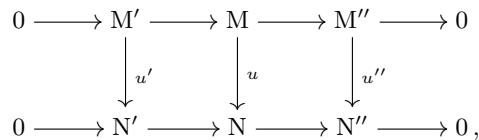
\includegraphics[keepaspectratio]{images/part002_92bb4337.jpg}}

where the first (resp. second) line is an exact sequence of Z{[}G{]}-modules (resp. of Z{[}H{]}-modules) and where \(u', u, u''\) are compatible with \(\varphi\) . Prove that the diagram

\[
\begin{array}{l} \dots \longrightarrow \mathrm{H} ^ {n} (\mathrm{G}, \mathrm{M} ^ {\prime}) \longrightarrow \mathrm{H} ^ {n} (\mathrm{G}, \mathrm{M}) \longrightarrow \mathrm{H} ^ {n} (\mathrm{G}, \mathrm{M} ^ {\prime \prime}) \longrightarrow \mathrm{H} ^ {n + 1} (\mathrm{G}, \mathrm{M} ^ {\prime}) \longrightarrow \dots \\ \Biggl \downarrow_ {\mathrm{H} ^ {n} (\varphi , u ^ {\prime})} \qquad \Biggl \downarrow_ {\mathrm{H} ^ {n} (\varphi , u)} \qquad \Biggl \downarrow_ {\mathrm{H} ^ {n} (\varphi , u ^ {\prime \prime})} \qquad \Biggl \downarrow_ {\mathrm{H} ^ {n + 1} (\varphi , u)} \\ \dots \longrightarrow \mathrm{H} ^ {n} (\mathrm{H}, \mathrm{N} ^ {\prime}) \longrightarrow \mathrm{H} ^ {n} (\mathrm{H}, \mathrm{N}) \longrightarrow \mathrm{H} ^ {n} (\mathrm{H}, \mathrm{N} ^ {\prime \prime}) \longrightarrow \mathrm{H} ^ {n + 1} (\mathrm{H}, \mathrm{N} ^ {\prime}) \longrightarrow \dots \end{array}
\]

(whose horizontal lines are the long exact sequences defined in Exercise 1, c)) is commutative.

\begin{enumerate}
\def\labelenumi{\alph{enumi})}
\setcounter{enumi}{3}
\item
  Examples: If H = G, then the mapping u is compatible with \(Id_{G}\) if and and only if it is Z{[}G{]}-linear, and we have \(\mathrm{H}^{n}(\mathrm{Id}_{\mathrm{G}}, u) = \mathrm{H}^{n}(\mathrm{G}, u)\) . If N is equal to M endowed with the Z{[}G{]}-module structure deduced from \(\varphi\) , then the homomorphisms \(\varphi\) and \(1_{M}\) are compatible; we denote by \(\operatorname{Res}^{q} : \mathrm{H}^{q}(\mathrm{G}, \mathrm{M}) \to \mathrm{H}^{q}(\mathrm{H}, \mathrm{M})\) the homomorphism \(\mathrm{H}^{q}(\varphi, 1_{\mathrm{M}})\) (``restriction homomorphism'').
\item
  Let H be a normal subgroup of G, and let \(M^{H}\) be the subgroup of M consisting of the elements invariant under H, endowed with the action of G/H deduced from that of G by passing to the quotient. The canonical surjection \(p: G \rightarrow G/H\) and the canonical injection \(j: M^{H} \rightarrow M\) are compatible; we denote by \(\operatorname{Inf}^{q}: \operatorname{H}^{q}(\operatorname{G}/\operatorname{H}, \operatorname{M}^{\operatorname{H}}) \to \operatorname{H}^{q}(\operatorname{G}, \operatorname{M})\) the homomorphism \(\operatorname{H}^{q}(p, j)\) (``inflation homomorphism''). Prove that the sequence
\end{enumerate}

\[
0 \to \mathrm{H} ^ {1} (\mathrm{G} / \mathrm{H}, \mathrm{M} ^ {\mathrm{H}}) \xrightarrow {\operatorname{Inf} ^ {1}} \mathrm{H} ^ {1} (\mathrm{G}, \mathrm{M}) \xrightarrow {\operatorname{Res} ^ {1}} \mathrm{H} ^ {1} (\mathrm{H}, \mathrm{M})
\]

is exact. If, moreover, \(\mathrm{H}^1 (\mathrm{H},\mathrm{M})\) is zero, then the sequence

\[
0 \to \mathrm{H} ^ {2} (\mathrm{G} / \mathrm{H}, \mathrm{M} ^ {\mathrm{H}}) \xrightarrow {\operatorname{Inf} ^ {2}} \mathrm{H} ^ {2} (\mathrm{G}, \mathrm{M}) \xrightarrow {\operatorname{Res} ^ {2}} \mathrm{H} ^ {2} (\mathrm{H}, \mathrm{M})
\]

is exact.

¶ 3) Let G be a group and M a Z{[}G{]}-module. Let G act on C \(^{1}\) (G,M) by sending \((g,f)\in\mathrm{G}\times\mathrm{C}^{1}(\mathrm{G},\mathrm{M})\) to the function \(h\mapsto gf(g^{-1}h)\) on G. Recall (I, §6, p.~149, Exercise 8) that a G-mean on M is a Z{[}G{]}-linear mapping \(\mu:C^{1}(\mathrm{G},\mathrm{M})\to\mathrm{M}\) satisfying \(\mu(c_{x})=x\) , where \(c_{x}\) denotes the constant function with value \(x\in\mathrm{M}\) .

\begin{enumerate}
\def\labelenumi{\alph{enumi})}
\item
  Prove that if M admits a G-mean, then \(\mathrm{H}^{n}(\mathrm{G},\mathrm{M})\) is zero for \(n \geqslant 1\) . (For \(q \geqslant 1\) , let \(h^{q}: \mathrm{C}^{q}(\mathrm{G},\mathrm{M}) \to \mathrm{C}^{q-1}(\mathrm{G},\mathrm{M})\) be the following homomorphism: for \(g_{1}, \ldots, g_{q-1}\) in G and \(c \in \mathrm{C}^{q}(\mathrm{G}, \mathrm{M})\) , define \(h^{q}(c)(g_{1}, \ldots, g_{q-1})\) as the image by \(\mu\) of the function \(g \mapsto c(g_{1}, \ldots, g_{q-1}, (g_{1} \cdots g_{q-1})^{-1}g)\) . Prove the equality \(h^{q+1} \circ d^{q} + d^{q-1} \circ h^{q} = 1_{\mathrm{C}^{q}(\mathrm{G}, \mathrm{M})}\) .
\item
  Let A be an abelian group; denote by \(\mathcal{F}(\mathrm{G},\mathrm{A})\) the group of mappings from G to A, endowed with the action of G defined by \({}^{g}f(h)=f(hg)\) for g,h in G and f in \(\mathcal{F}(\mathrm{G},\mathrm{A})\) . For any mapping c from G to \(\mathcal{F}(\mathrm{G},\mathrm{A})\) , denote by \(\mu(c)\) the mapping \(g\mapsto c(g^{-1})(g)\) from G to A. Show that \(\mu\) is a G-mean on \(\mathcal{F}(\mathrm{G},\mathrm{A})\) ; we therefore have \(\mathrm{H}^{q}(\mathrm{G},\mathcal{F}(\mathrm{G},\mathrm{A}))=0\) for \(q\geqslant1\) .
\item
  Let \(j: M \to \mathcal{F}(G, M)\) be the mapping that sends an element m of M to the function \(g \mapsto gm\) , and let \(M'\) be its cokernel. Prove that j is injective and Z{[}G{]}-linear. Deduce that the homomorphism \(\partial^{q}: H^{q}(G, M') \to H^{q+1}(G, M)\) is bijective for \(q \geqslant 1\) .
\item
  Let L be a finite Galois extension of the commutative field K and G be its Galois group. Deduce from b) and the normal basis theorem (V, §10, No.~9, p.~73) that the groups \(\mathrm{H}^{n}(\mathrm{G},\mathrm{L})\) are zero for \(n \geqslant 1\) .
\end{enumerate}

¶ 4) Let G be a group and H a subgroup of G. For any Z{[}H{]}-module N, denote by \(\widetilde{N}\) the group \(\operatorname{Hom}_{\mathbf{Z}[H]}(\mathbf{Z}[G], N)\) endowed with a Z{[}G{]}-module structure deduced from the right Z{[}G{]}-module structure on Z{[}G{]}.

\begin{enumerate}
\def\labelenumi{\alph{enumi})}
\item
  Prove that \(\widetilde{\mathbf{N}}\) can be identified with the \(\mathbf{Z}[\mathrm{G}]\) -submodule of \(\mathcal{F}(\mathrm{G},\mathrm{N})\) (Exercise 3) consisting of the mappings \(f\) such that \(f(hg) = hf(g)\) for every \(h\in \mathrm{H}\) and \(g\in \mathrm{G}\) . If \(\mathrm{A}\) is an abelian group, then the \(\mathbf{Z}[\mathrm{G}]\) -module \(\widetilde{\mathcal{F}(\mathrm{H},\mathrm{A})}\) is canonically isomorphic to \(\mathcal{F}(\mathrm{G},\mathrm{A})\) .
\item
  Let \(0 \rightarrow N' \stackrel{i}{\rightarrow} N \stackrel{p}{\rightarrow} N'' \rightarrow 0\) be an exact sequence of Z{[}H{]}-modules; the sequence
\end{enumerate}

\[
0 \longrightarrow \widetilde {\mathrm{N}} ^ {\prime} \xrightarrow {\operatorname{Hom} (1 , i)} \widetilde {\mathrm{N}} \xrightarrow {\operatorname{Hom} (1 , p)} \widetilde {\mathrm{N}} ^ {\prime \prime} \longrightarrow 0
\]

is exact (observe that the \(\mathbf{Z}[\mathrm{H}]\) -module \(\mathbf{Z}[\mathrm{G}]\) is free).

\begin{enumerate}
\def\labelenumi{\alph{enumi})}
\setcounter{enumi}{2}
\tightlist
\item
  Let \(u_{N} : \widetilde{N} \to N\) be the mapping \(f \mapsto f(1)\) ; it is compatible with the canonical injection \(i : H \to G\) (Exercise 2). Prove that the homomorphism
\end{enumerate}

\[
\mathrm{H} ^ {q} (i, u _ {\mathrm{N}}): \mathrm{H} ^ {q} (\mathrm{G}, \widetilde {\mathrm{N}}) \to \mathrm{H} ^ {q} (\mathrm{H}, \mathrm{N})
\]

is bijective for every \(q \geqslant 0\) (first treat the case q = 0 and then reason by induction on q using the above; Exercise 3, c); and Exercise 2, c)).

\begin{enumerate}
\def\labelenumi{\alph{enumi})}
\setcounter{enumi}{3}
\item
  Suppose that H has finite index n in G. Let M be a Z{[}G{]}-module, which we view as a Z{[}H{]}-module by restriction of scalars. Let \(f \in \widetilde{M}\) ; the element \(g^{-1}f(g)\) depends only on the right class Hg of g. Set \(\pi(f) = \sum_{Hg \in H \setminus G} g^{-1}f(g)\) . Prove that \(\pi\) is a Z{[}G{]}-linear homomorphism from \(\widetilde{M}\) to M. For any integer \(q \geqslant 0\) , denote by \(\operatorname{Cor}^{q}: \mathrm{H}^{q}(\mathrm{H}, \mathrm{M}) \to \mathrm{H}^{q}(\mathrm{G}, \mathrm{M})\) the homomorphism \(\mathrm{H}^{q}(\pi) \circ \mathrm{H}^{q}(i, u_{\mathrm{M}})^{-1}\) (``corestriction homomorphism'').
\item
  Prove that the endomorphism \(Cor^{q} \circ Res^{q}\) of \(H^{q}(G, M)\) is multiplication by n (first treat the case q = 0 and then treat the general case as in the proof of c)).
\item
  Suppose that G is finite; prove that for every Z{[}G{]}-module M and every integer \(q \geqslant 1\) , the group \(\mathrm{H}^{q}(\mathrm{G}, \mathrm{M})\) is annihilated by the order of G.
\end{enumerate}

\begin{enumerate}
\def\labelenumi{\arabic{enumi})}
\setcounter{enumi}{4}
\tightlist
\item
  Let G be a group and M a not necessarily abelian group endowed with a homomorphism \(\varphi: G \to \text{Aut}(M)\) ; for \(g \in G\) and \(m \in M\) , set \(^{g}m = \varphi(g)(m)\) . Denote by \(H^{0}(G, M)\) the subgroup of M consisting of the elements fixed by the action of G; its identity element is called the marked or distinguished element of \(H^{0}(G, M)\) . Let \(Z^{1}(G, M)\) be the set of mappings \(c: G \to M\) satisfying \(c(gh) = c(g)^{g}c(h)\) for g, h in G. For \(c \in Z^{1}(G, M)\) and \(m \in M\) , the mapping \(g \mapsto mc(g)(^g m)^{-1}\) belongs to \(Z^{1}(G, M)\) ; this defines an action of the group M on \(Z^{1}(G, M)\) . The quotient set is denoted by \(H^{1}(G, M)\) ; it is endowed with a marked element, namely the class of the constant mapping with value 1. If M is abelian, then the set \(H^{1}(G, M)\) coincides with that defined in Exercise 1.
\end{enumerate}

\begin{enumerate}
\def\labelenumi{\alph{enumi})}
\item
  Let N be a second group endowed with an action of G and \(u: M \to N\) a group homomorphism compatible with the actions of G. For i = 0, 1, define homomorphisms \(\mathrm{H}^{i}(u): \mathrm{H}^{i}(\mathrm{G}, \mathrm{M}) \to \mathrm{H}^{i}(\mathrm{G}, \mathrm{N})\) that send the marked element of \(\mathrm{H}^{i}(\mathrm{G}, \mathrm{M})\) to that of \(\mathrm{H}^{i}(\mathrm{G}, \mathrm{N})\) .
\item
  Let \(0 \to M' \xrightarrow{\iota} M \xrightarrow{\pi} M'' \to 0\) be an exact sequence of groups with operators in G. Let \(x'' \in \mathrm{H}^0(\mathrm{G}, \mathrm{M}'')\) , and let x be an element of M such that \(\pi(x) = x''\) . Prove that there exists an element \(c' \in \mathrm{Z}^1(\mathrm{G}, \mathrm{M}')\) such that \(\iota \circ c'(g) = g^{-1}c(g)\) for every \(g \in G\) and that the class of \(c'\) in \(\mathrm{H}^1(\mathrm{G}, \mathrm{M}')\) depends only on \(x''\) ; we denote that class by \(\partial(x'')\) . Prove that the sequence
\end{enumerate}

\[
0 \to \mathrm{H} ^ {0} (\mathrm{G}, \mathrm{M} ^ {\prime}) \xrightarrow {\mathrm{H} ^ {0} (\iota)} \mathrm{H} ^ {0} (\mathrm{G}, \mathrm{M}) \xrightarrow {\mathrm{H} ^ {0} (\pi)} \mathrm{H} ^ {0} (\mathrm{G}, \mathrm{M} ^ {\prime \prime}) \xrightarrow {\partial}
\]

\[
\mathrm{H} ^ {1} (\mathrm{G}, \mathrm{M} ^ {\prime}) \xrightarrow {\mathrm{H} ^ {1} (\iota)} \mathrm{H} ^ {1} (\mathrm{G}, \mathrm{M}) \xrightarrow {\mathrm{H} ^ {1} (\pi)} \mathrm{H} ^ {1} (\mathrm{G}, \mathrm{M} ^ {\prime \prime})
\]

is exact (a sequence of mappings \(G \xrightarrow{i} F \xrightarrow{p} E\) , where the set E is endowed with a marked element e, is called exact in F if \(\operatorname{Im}(i) = p^{-1}(e)\) ).

\begin{enumerate}
\def\labelenumi{\alph{enumi})}
\setcounter{enumi}{2}
\item
  Suppose, moreover, that \(M'\) is contained in the center of M. Construct a mapping \(\partial^{1}: H^{1}(G, M'') \to H^{2}(G, M')\) such that the inverse image of the identity element by \(\partial^{1}\) is the image of \(H^{1}(\pi)\) . Also define an action of the group \(H^{1}(G, M')\) on the set \(H^{1}(G, M)\) such that two elements are conjugate for this action if and only if they have the same image by \(H^{1}(\pi)\) .
\item
  Let K be a commutative field, L a finite Galois extension of K with Galois group G, and n an integer. Let G act on the group \(\mathbf{GL}_{n}(\mathrm{L})\) by setting \(\sigma A = (\sigma(a_{ij}))\) for \(\sigma \in G\) and \(A = (a_{ij}) \in \mathbf{GL}_{n}(\mathrm{L})\) . Deduce from V, §10, No.~5, p.~64, Proposition 9 that the set \(\mathrm{H}^{1}(\mathrm{G}, \mathbf{GL}_{n}(\mathrm{L}))\) is reduced to one element (``Hilbert's 90 theorem'').
\end{enumerate}

¶ 6) Let L be a finite Galois extension of the commutative field K, with Galois group G. Let V and V' be K-vector spaces and w (resp. w') a tensor of type \((p,q)\) on V (resp. V'). An L-isomorphism from \((V,w)\) to \((V',w')\) is an L-linear isomorphism \(u:V_{(L)}\to V_{(L)}'\) such that \(u^{\otimes p}\otimes(^{t}u^{-1})^{\otimes q}\) sends the image of w to that of \(w'\) . We denote by \(\operatorname{Aut}_{\mathrm{L}}(\mathrm{V},w)\) the group of L-automorphisms of \((\mathrm{V},w)\) , on which G acts by \(\sigma\varphi=(1_{\mathrm{V}}\otimes\sigma)\circ\varphi\circ(1_{\mathrm{V}}\otimes\sigma)^{-1}\) .

\begin{enumerate}
\def\labelenumi{\alph{enumi})}
\item
  Let u be an L-isomorphism from \((\mathrm{V}, w)\) to \((\mathrm{V}^{\prime}, w^{\prime})\) and \(\sigma\) an element of G; the mapping \(\sigma u = (1_{\mathrm{V}^{\prime}} \otimes \sigma) \circ u \circ (1_{\mathrm{V}} \otimes \sigma)^{-1}\) is an L-isomorphism from \((\mathrm{V}, w)\) to \((\mathrm{V}^{\prime}, w^{\prime})\) , so that \(c(\sigma) = u^{-1} \circ \sigma u\) is an element of \(\operatorname{Aut}_{\mathrm{L}}(\mathrm{V}, w)\) . Prove that the mapping \(c : G \to \operatorname{Aut}_{\mathrm{L}}(\mathrm{V}, w)\) belongs to \(Z^{1}(\mathrm{G}, \operatorname{Aut}_{\mathrm{L}}(\mathrm{V}, w))\) and that its class \(\theta(\mathrm{V}^{\prime}, w^{\prime})\) in \(H^{1}(\mathrm{G}, \operatorname{Aut}_{\mathrm{L}}(\mathrm{V}, w))\) does not depend on the choice of u.
\item
  Prove that the mapping \((\mathrm{V}^{\prime},t^{\prime})\mapsto\theta(\mathrm{V}^{\prime},t^{\prime})\) defines a bijection from the set of K-isomorphism classes of pairs \((\mathrm{V}^{\prime},w^{\prime})\) L-isomorphic to \((\mathrm{V},w)\) to the set \(\mathrm{H}^{1}(\mathrm{G},\mathrm{Aut}_{\mathrm{L}}(\mathrm{V},w))\) . (Given an element c of \(\mathrm{Z}^{1}(\mathrm{G},\mathrm{Aut}_{\mathrm{L}}(\mathrm{V},w))\) , deduce from Exercise 5, d) an L-automorphism f of \(\mathrm{V}_{(\mathrm{L})}\) such that \(c(\sigma)=f^{-1}\circ^{\sigma}f\) . Prove that the image \(w^{\prime}\) of w by the automorphism deduced from f is rational over K, and consider the pair \((\mathrm{V},w^{\prime}).\) )
\end{enumerate}

* c) Examples: The set \(\mathrm{H}^1 (\mathrm{G},\mathbf{Sp}_{2n}(\mathrm{L}))\) is reduced to one element. If Q is a quadratic form on K, then the set \(\mathrm{H}^1 (\mathrm{G},\mathbf{O}(\mathrm{Q}_{(\mathrm{L})}))\) can be identified with the set of equivalence classes of quadratic forms on K equivalent to Q over L.*

\(d\) ) Let A be a K-algebra and M the automorphism group of the L-algebra \(\mathrm{A}_{(\mathrm{L})}\) , endowed with the action of G defined above. The construction in \(b\) ) defines a bijection from the set of isomorphism classes of pairs \((\mathrm{B},u)\) , where B is a K-algebra and \(u\) is an isomorphism from \(\mathrm{B}_{(\mathrm{L})}\) to \(\mathrm{A}_{(\mathrm{L})}\) , to the set \(Z^{1}(\mathrm{G},\mathrm{M})\) . The inverse bijection sends an element \(c\) of \(Z^{1}(\mathrm{G},\mathrm{M})\) to the K-subalgebra of \(\mathrm{A}_{(\mathrm{L})}\) consisting of the elements \(a\) satisfying \(c(\sigma)(\sigma(a)) = a\) for every \(\sigma \in \mathrm{G}\) .

\begin{enumerate}
\def\labelenumi{\arabic{enumi})}
\setcounter{enumi}{6}
\tightlist
\item
  Let L be an extension of K. For any integer \(n \geqslant 1\) , denote by \(\mathcal{A}_{n}(\mathrm{L}/\mathrm{K})\) the set of isomorphism classes of central simple K-algebras of degree \(n^{2}\) split by L.
\end{enumerate}

\begin{enumerate}
\def\labelenumi{\alph{enumi})}
\item
  Prove that the kernel \(\mathrm{Br}(\mathrm{L} / \mathrm{K})\) of the canonical homomorphism \(\mathrm{Br}(\mathrm{K})\to \mathrm{Br}(\mathrm{L})\) is isomorphic to the direct limit of the sets \(\mathcal{A}_n(\mathrm{L} / \mathrm{K})\) ; specify a system of mappings. b) Assume from now on that L is a finite Galois extension of K, with Galois group G. Deduce a bijection \(\theta_{n}:\mathcal{A}_{n}(\mathrm{L} / \mathrm{K})\to \mathrm{H}^{1}(\mathrm{G},\mathbf{PGL}_{n}(\mathrm{L}))\) from Exercise 6.
\item
  Denote by \(\partial_n: \mathrm{H}^1(\mathrm{G}, \mathbf{PGL}_n(\mathrm{L})) \to \mathrm{H}^2(\mathrm{G}, \mathrm{L}^*)\) the mapping deduced from the exact sequence \(1 \to \mathrm{L}^* \to \mathbf{GL}_n(\mathrm{L}) \to \mathbf{PGL}_n(\mathrm{L}) \to 1\) (Exercise 5, c)) and by \(\delta_n: \mathcal{A}_n(\mathrm{L/K}) \to \mathrm{H}^2(\mathrm{G}, \mathrm{L}^*)\) the mapping \(\partial_n \circ \theta_n\) . If \(\mathrm{A} \in \mathcal{A}_n(\mathrm{L/K})\) , then we have \(\delta_n(\mathrm{A}) = 0\) if and only if \(\mathrm{A}\) is a matrix algebra over \(\mathrm{K}\) ; if \(\mathrm{A} \in \mathcal{A}_p(\mathrm{L/K})\) and \(\mathrm{B} \in \mathcal{A}_q(\mathrm{L/K})\) , then we have \(\delta_{pq}(\mathrm{A} \otimes_{\mathrm{K}} \mathrm{B}) = \delta_p(\mathrm{A}) + \delta_q(\mathrm{B})\) . Deduce an injective group homomorphism \(\delta_{\mathrm{L/K}}: \mathrm{Br}(\mathrm{L/K}) \to \mathrm{H}^2(\mathrm{G}, \mathrm{L}^*)\) by passing to the direct limit. d) Prove that \(\partial_n\) is surjective for \(n = \operatorname{Card}(\mathrm{G})\) . (Let \(c: \mathrm{G} \times \mathrm{G} \to \mathrm{L}^*\) be an element of \(\mathrm{Z}^2(\mathrm{G}, \mathrm{L}^*)\) . For every \(\sigma \in \mathrm{G}\) , consider the endomorphism \(u(\sigma)\) of \(\mathrm{L}^{\mathrm{G}}\) that sends \(e_\tau\) to \(c(\sigma, \tau)e_{\sigma\tau}\) for every \(\tau \in \mathrm{G}\) , and determine \(u(\sigma)^{\sigma}u(\tau)u(\sigma\tau)^{-1}\) .)
\item
  Compare \(\delta_{\mathrm{L / K}}\) and \(\Phi_{\mathrm{L / K}}\) .
\item
  Prove that the group \(\mathrm{Br}(\mathrm{K})\) can be identified with the limit of the direct system of groups \(\left(\mathrm{H}^{2}(\mathrm{Gal}(\mathrm{L}/\mathrm{K}),\mathrm{L}^{*})\right)\) with respect to the set (ordered by inclusion) of finite Galois extensions of K contained in a fixed algebraic closure of K, where the homomorphisms between these groups are the (injective) inflation homomorphisms. g) Let F be an extension of K contained in L and \(\Gamma\) the subgroup of G that leaves F invariant. Prove that the following diagram commutes:
\end{enumerate}

\[
\begin{array}{c} \operatorname{Br} (\mathrm{L} / \mathrm{K}) \xrightarrow {r _ {\mathrm{F} / \mathrm{K}}} \operatorname{Br} (\mathrm{F} / \mathrm{L}) \\ \Biggl \downarrow_ {\delta_ {\mathrm{L} / \mathrm{K}}} \qquad \qquad \qquad \qquad \Biggl \downarrow_ {\delta_ {\mathrm{F} / \mathrm{L}}} \\ \operatorname{H} ^ {2} (\operatorname{G}, \operatorname{L} ^ {*}) \xrightarrow {\operatorname{Res} ^ {2}} \operatorname{H} ^ {2} (\Gamma , \operatorname{L} ^ {*}). \end{array}
\]

Deduce a canonical isomorphism from \(\mathrm{Br}(\mathrm{F}/\mathrm{K})\) to the kernel of the homomorphism \(\mathrm{Res}^{2}:\mathrm{H}^{2}(\mathrm{G},\mathrm{L}^{*})\to\mathrm{H}^{2}(\Gamma,\mathrm{L}^{*})\) .

\begin{enumerate}
\def\labelenumi{\arabic{enumi})}
\setcounter{enumi}{7}
\item
  Let L be an extension of K. Suppose that K has characteristic p \textgreater{} 0 and \(L = K^{1/p}\) . Prove that the group \(\mathrm{Br}(\mathrm{L}/\mathrm{K})\) is equal to the kernel of multiplication by p in \(\mathrm{Br}(\mathrm{K})\) (observe that if N is a finite Galois extension of K, then \(N^{1/p}\) is a Galois extension of L with the same Galois group).
\item
  Let G be a finite group and M a Z{[}G{]}-module. Denote by \(N_{G}\) the homomorphism \(m \mapsto \sum_{g} gm\) from M to M; its image is contained in the submodule \(M^{G}\) of M consisting of the invariant elements. Let \(\mathrm{T}_{\mathrm{G}}(\mathrm{M})\) be the quotient group \(\mathrm{M}^{\mathrm{G}}/\mathrm{N}_{\mathrm{G}}(\mathrm{M})\) . a) Let \(c \in \mathrm{Z}^{2}(\mathrm{G}, \mathrm{M})\) . Prove that the element \(\sum_{h} c(h, g)\) belongs to \(M^{G}\) ; we denote its class in \(\mathrm{T}_{\mathrm{G}}(\mathrm{M})\) by \(\theta_{c}(g)\) . Prove that \(\theta_{c}\) is a homomorphism from G to \(\mathrm{T}_{\mathrm{G}}(\mathrm{M})\) that is zero when \(c \in \mathrm{B}^{2}(\mathrm{G}, \mathrm{M})\) . Deduce a homomorphism \(\theta_{\mathrm{M}} : \mathrm{H}^{2}(\mathrm{G}, \mathrm{M}) \to \mathrm{Hom}(\mathrm{G}, \mathrm{T}_{\mathrm{G}}(\mathrm{M}))\) from it.
\end{enumerate}

\begin{enumerate}
\def\labelenumi{\alph{enumi})}
\setcounter{enumi}{1}
\tightlist
\item
  Let \(u: M \to N\) be a homomorphism of Z{[}G{]}-modules and \(\widetilde{u}: T_{G}(M) \to T_{G}(N)\) the homomorphism induced by u. Prove that we have \(\theta_{\mathrm{N}} \circ \mathrm{H}^{2}(u) = \mathrm{Hom}(1_{\mathrm{G}}, \widetilde{u}) \circ \theta_{\mathrm{M}}\) . c) Assume from now on that G is cyclic; let \(\sigma\) be a generator of G, and denote its order by n.~Let \(\chi \in \mathrm{Hom}(G, \mathbf{Z}/n\mathbf{Z})\) be the homomorphism that sends \(\sigma\) to the class of 1, and let \(\lambda \in H^{2}(G, \mathbf{Z})\) be its image by the connecting homomorphism associated with the exact sequence \(0 \to Z \to Z \to Z/nZ \to 0\) . Prove that \(\lambda\) is the class of the element \(\varepsilon \in Z^{2}(G, \mathbf{Z})\) such that for \(0 \leqslant p < n\) and \(0 \leqslant q < n\) , the image \(\varepsilon(\sigma^{p}, \sigma^{q})\) is equal to 0 if \(p + q < n\) and to 1 if \(p + q \geqslant n\) . For \(m \in M^{G}\) , denote by \(h_{m}\) the Z{[}G{]}-linear mapping from Z to M such that \(h_{m}(1) = m\) . Prove that the image of \(H^{2}(h_{m})(\lambda)\) by \(\theta_{M}\) is equal to the class of m, so that \(\theta_{M}\) is surjective.
\end{enumerate}

\(d\) ) Prove that \(\theta_{\mathrm{M}}\) is an isomorphism. (Let \(c\in \mathbf{Z}^2 (\mathrm{G},\mathrm{M})\) . Prove that we may assume \(c(g,1) = c(1,g) = 1\) for every \(g\in \mathrm{G}\) , and determine the images by \(d^1\) of the elements \(b\) and \(a_{m}\) \((m\in \mathrm{M})\) of \(\mathrm{C}^1 (\mathrm{G},\mathrm{M})\) defined by \(b(\sigma^{p}) = \sum_{i = 0}^{p - 1}c(\sigma^{i},\sigma)\) and \(a_{m}(\sigma^{p}) = \sum_{i = 0}^{p - 1}\sigma^{i}m.)\)

\begin{enumerate}
\def\labelenumi{\arabic{enumi})}
\setcounter{enumi}{9}
\tightlist
\item
  \begin{enumerate}
  \def\labelenumii{\alph{enumii})}
  \tightlist
  \item
    Let L be a cyclic extension of K. Deduce from Exercises 9 and 7 that the groups Br(L/K) and \(K^{*}/N_{L/K}(L^{*})\) are isomorphic.
  \end{enumerate}
\end{enumerate}

\begin{enumerate}
\def\labelenumi{\alph{enumi})}
\setcounter{enumi}{1}
\item
  Suppose that every extension L of K of finite degree is cyclic and that the norm mapping \(N_{L/K}: L^{*} \to K^{*}\) is surjective. Prove that every field extension of K of finite degree with center K is equal to K.
\item
  Apply the previous question to finite fields.
\end{enumerate}

\begin{enumerate}
\def\labelenumi{\arabic{enumi})}
\setcounter{enumi}{10}
\tightlist
\item
  Let L be a cyclic extension of K with Galois group G, and let \(\sigma\) be a generator of G. Exercise 10 gives a canonical isomorphism \(\mathrm{Br}(\mathrm{L}/\mathrm{K}) \to \mathrm{K}^{*}/\mathrm{N}_{\mathrm{L}/\mathrm{K}}(\mathrm{L}^{*})\) , whose inverse we will now construct explicitly.
\end{enumerate}

Let \(\theta \in \mathrm{K}^*\) , and let \(c_{\theta} \in \mathrm{Z}^{2}(\mathrm{G}, \mathrm{L}^{*})\) be the element defined by \(c_{\theta}(\sigma^{p}, \sigma^{q}) = \theta^{\varepsilon(p,q)}\) (Exercise 9, \(c\) )). Prove that the cross product A{[} \(\mathcal{E}\) , L{]} of L and the extension \(\mathcal{E}\) associated with \(c_{\theta}\) is isomorphic to the quotient of the K-algebra L{[}X{]} \(_{\sigma}\) (VIII, p.~11) by the (two-sided) ideal generated by the central element X \(^{n}\) - \(\theta\) . The class of A \(_{\theta}\) in Br(L/K) corresponds to the class of \(\theta\) ( \(\text{mod } \mathrm{N}_{\mathrm{L/K}}(\mathrm{L}^{*})\) ) by the isomorphism defined above.

\begin{enumerate}
\def\labelenumi{\arabic{enumi})}
\setcounter{enumi}{11}
\tightlist
\item
  Let A be a commutative ring. Endow the set of isomorphism classes of Azumaya A-algebras (VIII, p.~270, Exercise 8) with the structure of a monoid by setting \(\operatorname{cl}(S)\operatorname{cl}(T)=\operatorname{cl}(S\otimes_{A}T)\) .
\end{enumerate}

\begin{enumerate}
\def\labelenumi{\alph{enumi})}
\item
  Prove that the quotient monoid for Morita equivalence is an abelian group; we denote it by Br(A) and call it the Brauer group of A (when A is a field, this definition coincides with that given in VIII, p.~279). Denote by {[}S{]} the class of an Azumaya A-algebra S in Br(A). The identity element of Br(A) is the class of A, and the inverse of an element {[}S{]} is {[}S°{]}.
\item
  Let S be an Azumaya A-algebra. We have \([S] = [A]\) if and only if there exists a finitely generated, projective, faithful A-module P such that S is isomorphic to \(\operatorname{End}_{\mathrm{A}}(\mathrm{P})\) .
\item
  Let B be a commutative A-algebra. Define a group homomorphism \(r_{B/A} : \mathrm{Br}(A) \to \mathrm{Br}(B)\) such that \(r_{\mathrm{B/A}}([\mathrm{S}]) = [\mathrm{S}_{(\mathrm{B})}]\) for every Azumaya A-algebra S. We denote the kernel of this homomorphism by \(\mathrm{Br(B/A)}\) .
\end{enumerate}

¶ 13) Let A be a commutative ring, B a commutative A-algebra, and G a finite group of automorphisms of the A-algebra B. Suppose that B is a finitely generated, projective, faithful A-module and that the A-linear homomorphism \(\psi : \mathrm{B} \otimes_{\mathrm{A}} \mathrm{B} \to \mathrm{B}^{\mathrm{G}}\) defined by \(\psi(b \otimes b') = (\sigma(b)b')_{\sigma \in \mathrm{G}}\) is bijective.

\begin{enumerate}
\def\labelenumi{\alph{enumi})}
\item
  Let N be a B-module, endowed with a homomorphism \(\sigma \mapsto u_{\sigma}\) from G to \(\mathrm{Aut}_{\mathrm{A}}(\mathrm{N})\) satisfying \(u_{\sigma}(bx) = \sigma(b)u_{\sigma}(x)\) for \(\sigma \in \mathrm{G}\) , \(b \in \mathrm{B}\) , \(x \in \mathrm{N}\) . Let M be the A-submodule of N consisting of the elements \(x\) such that \(u_{\sigma}(x) = x\) for every \(\sigma \in \mathrm{G}\) . Prove that the canonical B-homomorphism \(\mathrm{B} \otimes_{\mathrm{A}} \mathrm{M} \to \mathrm{N}\) is bijective (use Exercise 7, \(d\) ) of VIII, p.~270 to reduce to the case when B is the product algebra \(\mathrm{A}^{\mathrm{G}}\) on which G acts by permuting the factors).
\item
  Let S be an A-algebra and M the automorphism group of the B-algebra \(\mathrm{S}_{(\mathrm{B})}\) , on which G acts by \(\sigma\varphi = (\mathrm{Id}_{\mathrm{S}} \otimes \sigma) \circ \varphi \circ (\mathrm{Id}_{\mathrm{S}} \otimes \sigma)^{-1}\) . Extend the construction of Exercise 6 to define a bijection from the set of isomorphism classes of pairs \((T,u)\) , where T is an A-algebra and u an isomorphism from \(T_{(B)}\) to \(S_{(B)}\) , to the set \(Z^{1}(G,M)\) , as well as a bijection from the set of isomorphism classes of A-algebras T such that the B-algebras \(T_{(B)}\) and \(S_{(B)}\) are isomorphic to \(H^{1}(G,M)\) .
\item
  Assume from now on that every projective B-module is free. Adapt the reasoning of Exercise 8 to construct an isomorphism \(\theta : \mathrm{Br}(\mathrm{B} / \mathrm{A}) \to \mathrm{H}^2(\mathrm{G}, \mathrm{B}^*)\) .
\end{enumerate}

¶ 14) Let A be a Noetherian commutative local ring, m its maximal ideal, \(\kappa\) the field A/m, and S an Azumaya algebra over A.

\begin{enumerate}
\def\labelenumi{\alph{enumi})}
\item
  Let \(e\) be an idempotent in S whose image in S/mS is an indecomposable idempotent. Deduce from Nakayama's lemma (cf.~VIII, p.~168, Exercise 16) that the canonical homomorphism \(S \to \mathrm{End}_{\mathrm{A}}(Se)\) is bijective.
\item
  Suppose that m is nilpotent \(^{*}\) (or, more generally, that A is complete for the m-adic topology) \(^{*}\) . Prove that the homomorphism \(r_{\kappa/A}: \mathrm{Br}(A) \to \mathrm{Br}(\kappa)\) is injective.
\end{enumerate}

* \(c\) ) Assume from now on that A is complete. Let L be a separable extension of \(\kappa\) of finite degree that is a splitting field for the \(\kappa\) -algebra S/mS. Let \(x\) be a primitive element of L, \(f\) its minimal polynomial, F a monic polynomial in A{[}X{]} whose image in \(\kappa\) {[}X{]} is \(f\) , and B = A{[}X{]}/(F). Prove that B is a local A-algebra, free and finitely generated as an A-module, with maximal ideal mB and residue field isomorphic to L; the B-algebra S \(_{(B)}\) is isomorphic to a matrix algebra.

\(d\) ) Suppose, moreover, that L is a Galois extension of \(\kappa\) , with Galois group G. Prove that the action of G on L lifts to an action on the A-algebra B (let \(G'\) be the automorphism group of this algebra; deduce from Hensel's lemma (Comm. Alg., III, §4, No.~3, p.~215, Theorem 1) that the natural homomorphism \(G' \to G\) is bijective). Deduce from Nakayama's lemma that the homomorphism \(\psi : B \otimes_A B \to B^G\) defined in Exercise 13 is bijective.

\begin{enumerate}
\def\labelenumi{\alph{enumi})}
\setcounter{enumi}{4}
\item
  Prove that the homomorphism \(\mathrm{H}^{q}(\pi):\mathrm{H}^{q}(\mathrm{G},\mathrm{B}^{*})\to\mathrm{H}^{q}(\mathrm{G},\mathrm{L}^{*})\) is bijective for every \(q\geqslant1\) . (For \(i\geqslant1\) , let \(U^{i}\) be the subgroup of elements b of \(B^{*}\) such that \(b\equiv1\) (mod \(m^{i}B\) ). Observe that the Z{[}G{]}-module \(U^{i}/U^{i+1}\) is isomorphic to \(m^{i}B/m^{i+1}B\) , hence to a power of L, and deduce from Exercise 5, d) that \(\mathrm{H}^{q}(\mathrm{G},\mathrm{U}^{i}/\mathrm{U}^{i+1})\) is zero for \(q\geqslant1\) . Let \(c\in\mathrm{Z}^{q}(\mathrm{G},\mathrm{U}^{1})\) . Construct, by induction, a sequence \((b_{n})\) with \(b_{n}\in\mathrm{Z}^{q-1}(\mathrm{G},\mathrm{U}^{n})\) such that \(c-d^{q-1}(\sum_{i=1}^{n}b_{i})\) belongs to \(\mathrm{Z}^{q}(\mathrm{G},\mathrm{U}^{n+1})\) . Conclude that \(\mathrm{H}^{q}(\mathrm{G},\mathrm{U}^{1})\) is zero for \(q\geqslant1\) .
\item
  Conclude that the canonical homomorphisms \(\mathrm{Br}(B/A)\to \mathrm{Br}(L/\kappa)\) and \(\mathrm{Br}(A)\to \mathrm{Br}(\kappa)\) are bijective.*
\end{enumerate}

\begin{enumerate}
\def\labelenumi{\arabic{enumi})}
\setcounter{enumi}{14}
\tightlist
\item
  *a) Let A be a regular integral domain (AC, X, §4, n° 2, p.~55) and K its field of fractions. The homomorphism \(r_{\mathrm{K / A}}: \mathrm{Br(A)} \to \mathrm{Br(K)}\) is injective (VIII, p.~271, Exercise 11).*
\end{enumerate}

\begin{enumerate}
\def\labelenumi{\alph{enumi})}
\setcounter{enumi}{1}
\tightlist
\item
  Prove that the ring \(A = \mathbf{Q}[X, Y]/(X^{2} + Y^{2})\) is an integral domain; let K be its field of fractions. Let H be the quaternion algebra of type \((-1, 0, -1)\) over Q, which is a field (cf.~III, §2, No.~5, p.~445). Prove that the class of the Azumaya
\end{enumerate}

A-algebra \(\mathrm{H}_{(\mathrm{A})}\) in \(\mathrm{Br}(\mathrm{A})\) is not zero but that \(\mathrm{H}_{(\mathrm{K})}\) is isomorphic to \(\mathbf{M}_{2}(\mathrm{K})\) , so that the homomorphism \(r_{K/A}\) is not injective (observe that K contains an element of square -1).

\begin{enumerate}
\def\labelenumi{\arabic{enumi})}
\setcounter{enumi}{15}
\tightlist
\item
  \begin{enumerate}
  \def\labelenumii{\alph{enumii})}
  \tightlist
  \item
    Prove that the homomorphism \(r_{\mathrm{K[X]}/\mathrm{K}} : \mathrm{Br}(\mathrm{K}) \to \mathrm{Br}(\mathrm{K}[\mathrm{X}])\) induces an isomorphism from \(\mathrm{Br}(\mathrm{K})\) to a direct factor of \(\mathrm{Br}(\mathrm{K}[\mathrm{X}])\) .
  \end{enumerate}
\end{enumerate}

\(^{*}b\) ) Suppose that the field K is perfect. Prove that \(r_{K[X]/K}\) is an isomorphism (deduce from Tsen's theorem (VIII, p.~360, Exercise 7) that \(\mathrm{Br}(\mathrm{K}[\mathrm{X}])\) is the union of the groups \(\mathrm{Br}(\mathrm{L}[\mathrm{X}]/\mathrm{K}[\mathrm{X}])\) , where L runs through the Galois extensions of K of finite degree, and then apply Exercise 13).

\begin{enumerate}
\def\labelenumi{\alph{enumi})}
\setcounter{enumi}{2}
\tightlist
\item
  Let A be a regular Q-algebra that is an integral domain. Prove that the homomorphism \(r_{\mathrm{A[X]}/\mathrm{A}} : \mathrm{Br}(\mathrm{A}) \to \mathrm{Br}(\mathrm{A}[\mathrm{X}])\) is bijective (use b) and Exercise 15 to prove that the homomorphism \(\mathrm{Br}(\mathrm{A}[\mathrm{X}]) \to \mathrm{Br}(\mathrm{A})\) deduced from the surjection \(\mathrm{P} \mapsto \mathrm{P}(0)\) is injective).*
\end{enumerate}

\(d\) ) Suppose that K has characteristic \(p > 0\) and is not perfect; let \(\theta \in \mathrm{K} - \mathrm{K}^p\) . View \(\mathrm{B} = \mathrm{K}[\mathrm{U}]\) as a K{[}X{]}-algebra via the homomorphism \(\rho : \mathrm{K}[\mathrm{X}] \to \mathrm{B}\) determined by \(\rho (\mathrm{X}) = \mathrm{U}^p - \mathrm{U}\) . Let \(\sigma\) be the automorphism of this K{[}X{]}-algebra such that \(\sigma (\mathrm{U}) = \mathrm{U} + 1\) , and let S be the quotient K{[}X{]}-algebra of B{[}V{]}\(_{\sigma}\) (VIII, p.~11) by the two-sided ideal B(\(V^{p} - \theta\)). Let L be a K{[}X{]}-algebra that is a commutative field. Prove that if the equation \(y^p - y = X\) has a solution in L, then S\(_{(L)}\) is a matrix algebra over L (let L' = L{[}t{]}/(\(t^{p} - \theta\)); consider the homomorphism S → End\(_{\mathrm{L}}\) (L') that sends V to the multiplication \(m_t\) by t and U to \(m_y\) - D, where D is the L-derivation of L' such that D(t) = t). In the opposite case, S\(_{(L)}\) is a central simple L-algebra; it is a matrix algebra if and only if \(\theta\) is the norm of an element of the extension L{[}Y{]}/(\(Y^{p} - Y - X\)) of L (apply Exercise 11).

Deduce that S is an Azumaya K{[}X{]}-algebra and that its class in \(\mathrm{Br}(\mathrm{K}[\mathrm{X}])\) does not come from \(\mathrm{Br}(\mathrm{K})\) (take \(L = K(X)\) ).

*17) Suppose that the field K is complete for a discrete valuation \(v\) , assumed normed (cf.~Exercise 12 of VIII, p.~272); denote the ring of \(v\) by A and its residue field by \(\kappa\) . The homomorphism \(r_{\kappa / \mathrm{A}}: \mathrm{Br}(\mathrm{A}) \to \mathrm{Br}(\kappa)\) is bijective (Exercise 14); denote by \(\iota: \mathrm{Br}(\kappa) \to \mathrm{Br}(\mathrm{K})\) the homomorphism \(r_{\mathrm{A / K}} \circ r_{\kappa / \mathrm{A}}^{-1}\) .

\begin{enumerate}
\def\labelenumi{\alph{enumi})}
\tightlist
\item
  Let L be an unramified Galois extension of K of finite degree, with Galois group G. Let B be the valuation ring of \(v_{L}\) extending v and \(\kappa_{L}\) be its residue field. The homomorphism \(\iota\) induces a homomorphism \(\iota_{\mathrm{L}} : \mathrm{Br}(\kappa_{\mathrm{L}}/\kappa) \to \mathrm{Br}(\mathrm{L}/\mathrm{K})\) . Construct a split exact sequence
\end{enumerate}

\[
0 \to \mathrm{Br} (\kappa_ {\mathrm{L}} / \kappa) \xrightarrow {\iota_ {\mathrm{L}}} \mathrm{Br} (\mathrm{L} / \mathrm{K}) \to \mathrm{H} ^ {2} (\mathrm{G}, \mathbf {Z}) \to 0,
\]

where Z is endowed with the trivial action of G (observe that the exact sequence of Z{[}G{]}-modules \(0 \rightarrow B^{*} \rightarrow L^{*} \xrightarrow{v_{L}} Z\) splits, and use Exercise 14).

\begin{enumerate}
\def\labelenumi{\alph{enumi})}
\setcounter{enumi}{1}
\item
  Let G be a group. Using the exact sequence \(0 \rightarrow Z \rightarrow Q \rightarrow Q/Z \rightarrow 0\) , prove that the linking homomorphism of Exercise 1 induces an isomorphism from \(\operatorname{Hom}(G, \mathbf{Q}/\mathbf{Z})\) to \(\mathrm{H}^{2}(\mathrm{G}, \mathbf{Z})\) .
\item
  Conclude that we have a split exact sequence
\end{enumerate}

\[
0 \to \mathrm{Br} (\kappa) \stackrel {\iota} {\to} \mathrm{Br} (\mathrm{K}) \to \Xi (\mathfrak {g}, \mathbf {Q} / \mathbf {Z}) \to 0,
\]

where g is the Galois group of a separable closure of \(\kappa\) over \(\kappa\) and \(\Xi(\mathfrak{g})\) is the group of continuous homomorphisms from g to Q/Z, endowed with the discrete topology (pass to the direct limit using Exercise 12 of VIII, p.~272 and the fact that every finite Galois extension of \(\kappa\) is the residue field extension of an unramified finite Galois extension of K, unique up to isomorphism).

\(d\) ) Deduce that \(\operatorname {Br}(\mathrm{K}) = \{0\}\) if \(\kappa\) is algebraically closed.

\begin{enumerate}
\def\labelenumi{\alph{enumi})}
\setcounter{enumi}{4}
\tightlist
\item
  Suppose that the field \(\kappa\) is finite, in other words, that K is a finite extension of a p-adic field or a field of formal power series over a finite field. Construct an isomorphism from \(\mathrm{Br}(\mathrm{K})\) to \(Q/Z\).*
\end{enumerate}

\section{Reduced Norms and Traces}

In this section, K is a commutative field and A a central simple K-algebra of finite degree. We denote the reduced degree of A by n.

\subsection{Complements on Characteristic Polynomials}

Let L be a commutative ring and M a free L-module of finite rank m. If u is an endomorphism of M and r a natural number, then we denote by \(c_{r}(u)\) the trace of the endomorphism \(\wedge^{r}(u)\) of the free L-module \(\wedge^{r}(\mathrm{M})\) . In particular, we have

\[
c _ {0} (u) = 1, \quad c _ {1} (u) = \mathrm{Tr} (u), \quad c _ {m} (u) = \det (u),\tag{1}
\]

and \(c_{r}(u) = 0\) for r \textgreater{} m. By Proposition 7 of III, §8, No.~4, p.~527, the mapping \(u \mapsto \det(u)\) from End(M) to L is a homogeneous polynomial mapping of degree m (IV, §5, No.~9, p.~55). More generally, for every integer r such that \(0 \leqslant r \leqslant m\) , the mapping \(c_{r}\) from End(M) to L is a homogeneous polynomial mapping of degree r; this follows from Proposition 10 of III, §8, No.~5, p.~529.

Let \(u\) be an endomorphism of \(M\) and \(\overline{u}\) the endomorphism of the \(L[X]\) -module \(M[X] = M \otimes_{L} L[X]\) deduced from \(u\) by extension of scalars (II, §5, No.~1, p.~277). Recall (III, §8, No.~11, p.~541, Definition 3 and (50)) that the characteristic polynomial of \(u\) is the determinant \(\chi_u(X)\) of the \(L[X]\) -endomorphism \(X - \overline{u}\) of \(M[X]\) and that we have the relation

\[
\chi_ {u} (\mathrm{X}) = \sum_ {r = 0} ^ {m} (- 1) ^ {r} c _ {r} (u) \mathrm{X} ^ {m - r}.\tag{2}
\]

PROPOSITION 1. --- Let L be a commutative ring, M a free L-module of finite rank \(m \geqslant 1\) , and u an endomorphism of M. There exists a unique endomorphism \(\widetilde{u}\) of M satisfying the relation

\[
\widetilde {u} (x) \wedge w = x \wedge \wedge^ {m - 1} (u) (w)\tag{3}
\]

for \(x\in \mathrm{M}\) and \(w\in \bigwedge^{m - 1}(\mathrm{M})\) . Moreover, we have the relations

\[
u \circ \widetilde {u} = \widetilde {u} \circ u = \det (u) _ {\mathrm{M}},\tag{4}
\]

\[
\det (\widetilde {u}) = \det (u) ^ {m - 1},\tag{5}
\]

\[
\widetilde {u} = \sum_ {r = 0} ^ {m - 1} (- 1) ^ {r} c _ {m - 1 - r} (u) u ^ {r}.\tag{6}
\]

Lemma 1. --- Let p be an integer such that \(0 \leqslant p \leqslant m\) . For any w in \(\wedge^{p}(\mathrm{M})\) , let \(h_{p}(w)\) be the linear mapping \(w' \mapsto w \wedge w'\) from \(\wedge^{m-p}(\mathrm{M})\) to \(\wedge^{m}(\mathrm{M})\) . The linear mapping \(h_{p}: w \mapsto h_{p}(w)\) from \(\wedge^{p}(\mathrm{M})\) to \(\operatorname{Hom}_{\mathrm{L}}(\wedge^{m-p}(\mathrm{M}), \wedge^{m}(\mathrm{M}))\) is an isomorphism.

Let \((e_{i})_{i\in\mathrm{I}}\) be a basis of M; we endow the set I with a total order. For any subset J of I, set \(e_{\mathrm{J}}=e_{i_{1}}\wedge\cdots\wedge e_{i_{r}}\) , where \((i_{1},\ldots,i_{r})\) is the sequence of elements of J in increasing order. The L-module \(\wedge^{m-p}(\mathrm{M})\) admits as a basis the elements \(e_{\mathrm{S}}\) , where S runs through the set of subsets of I with m-p elements; \(\wedge^{m}(\mathrm{M})\) has \(\{e_{\mathrm{I}}\}\) as a basis. Consequently, there exists a basis of \(\mathrm{Hom}_{\mathrm{L}}(\wedge^{m-p}(\mathrm{M}),\wedge^{m}(\mathrm{M}))\) consisting of linear mappings \(e_{\mathrm{J}}^{*}\) characterized by the formula

\[
e _ {\mathrm{J}} ^ {*} (e _ {\mathrm{S}}) = \left\{ \begin{array}{l l} e _ {\mathrm{I}} & \text {if } I = J\cup S, \\ 0 & \text {otherwise}, \end{array} \right.\tag{7}
\]

where J runs through the set of subsets of I with p elements. It follows from formula (20) of III, §7, No.~8, p.~519 that for every subset J of I with p elements, we have \(h_{p}(e_{\mathrm{J}}) \in \{e_{\mathrm{J}}^{*}, -e_{\mathrm{J}}^{*}\}\) ; since the elements \(e_{J}\) form a basis of \(\Lambda^{p}(\mathrm{M})\) , the linear mapping \(h_{p}\) is bijective.

Let us now prove Proposition 1. Let \(u\) and \(\widetilde{u}\) be endomorphisms of M. Relation (3) is equivalent to

\[
h _ {1} \circ \widetilde {u} = \operatorname{Hom} (\wedge^ {m - 1} (u) \cdot 1 _ {\bigwedge^ {m} (\mathrm{M})}) \circ h _ {1};\tag{8}
\]

the mapping \(h_{1}\) is an isomorphism from M to \(\operatorname{Hom}_{\mathrm{L}}(\wedge^{m-1}(\mathrm{M}),\wedge^{m}(\mathrm{M}))\) by Lemma 1. Consequently, for every endomorphism u of M, there exists a unique endomorphism \(\widetilde{u}\) of M satisfying relation (3).

Let \(x_{1},\ldots,x_{m}\) be elements of M. Let us replace x with \(u(x_{1})\) and w with \(x_{2}\wedge\cdots\wedge x_{m}\) in (3); we obtain

\[
\widetilde {u} (u (x _ {1})) \wedge x _ {2} \wedge \dots \wedge x _ {m} = u (x _ {1}) \wedge \dots \wedge u (x _ {m}) = \det (u) x _ {1} \wedge \dots \wedge x _ {m}.
\]

Consequently, \(h_1(\widetilde{u} \circ u(x_1)) = h_1(\det(u)x_1)\) , which gives the relation \(\widetilde{u} \circ u = \det(u)_\mathrm{M}\) by Lemma 1.

We denote by U the endomorphism \(X - \overline{u}\) of the L{[}X{]}-module M{[}X{]} (VIII, p.~335). By the above applied to U, there exists an endomorphism \(\widetilde{U}\) of the L{[}X{]}-module M{[}X{]} that satisfies the relations

\[
\widetilde {\mathrm{U}} (x _ {1}) \wedge x _ {2} \wedge \dots \wedge x _ {m} = x _ {1} \wedge (\mathrm{X} x _ {2} - u (x _ {2})) \wedge \dots \wedge (\mathrm{X} x _ {m} - u (x _ {m}))\tag{9}
\]

for \(x_{1},\ldots ,x_{m}\) in M and

\[
\widetilde {\mathrm{U}} \circ \mathrm{U} = \det (\mathrm{X} - \overline {{u}}) _ {\mathrm{M} [ \mathrm{X} ]}.\tag{10}
\]

Let us view \(\widetilde{\mathbf{U}}\) as an element of \(\operatorname{End}(\mathbf{M})[\mathbf{X}]\) (VIII, p.~9); by formula (9) and Lemma 1, it has degree \(\leqslant m - 1\) , so we can write it as

\[
\widetilde {\mathrm{U}} = \sum_ {r = 0} ^ {m - 1} (- 1) ^ {r} u _ {r} X ^ {m - 1 - r},\tag{11}
\]

where the \(u_{r}\) are endomorphisms of M. By formula (2), relation (10) gives the equality

\[
\left(\sum_ {r = 0} ^ {m - 1} (- 1) ^ {r} u _ {r} \mathrm{X} ^ {m - 1 - r}\right) (\mathrm{X} - u) = \sum_ {r = 0} ^ {m} (- 1) ^ {r} c _ {r} (u) \mathrm{X} ^ {m - r}\tag{12}
\]

in the ring \(\operatorname{End}(M)[X]\) . By identifying the coefficients of the monomials in X on each side, we obtain the relations

\[
u _ {r} + u _ {r - 1} \circ u = c _ {r} (u) _ {\mathrm{M}} \qquad \mathrm{for} 1 \leqslant r \leqslant m - 1\tag{13}
\]

and

\[
u _ {0} = c _ {0} (u) _ {\mathrm{M}}, \quad u _ {m - 1} \circ u = c _ {m} (u) _ {\mathrm{M}}.\tag{14}
\]

From this, we deduce

\[
u _ {m - 1} = \sum_ {r = 0} ^ {m - 1} (- 1) ^ {r} c _ {m - 1 - r} (u) u ^ {r}.\tag{15}
\]

Now, when we identify the constant terms, equalities (9) and (11) imply \(u_{m-1} = \widetilde{u}\) ; formula (6) follows.

In particular, \(\widetilde{u}\) belongs to the subalgebra of \(\operatorname{End}(\mathbf{M})\) generated by \(u\) and therefore commutes with \(u\) . We have already established the relation \(\widetilde{u} \circ u = \det(u)_{\mathrm{M}}\) ; formula (4) follows.

Finally, let \(x_{1},\ldots,x_{m}\) be elements of M. We replace x with \(x_{1}\) and w with \(\widetilde{u}(x_{2})\wedge\cdots\wedge\widetilde{u}(x_{m})\) in formula (3). This gives

\[
\begin{array}{c} \widetilde {u} (x _ {1}) \wedge \widetilde {u} (x _ {2}) \wedge \dots \wedge \widetilde {u} (x _ {m}) = x _ {1} \wedge u \circ (\widetilde {u} (x _ {2})) \wedge \dots \wedge u \circ (\widetilde {u} (x _ {m})) \\ = \det (u) ^ {m - 1} x _ {1} \wedge x _ {2} \wedge \dots \wedge x _ {m} \end{array}
\]

and therefore formula (5).

Remarks. --- 1) The endomorphism \(\widetilde{u}\) of M coincides with what we called the cotranspose of \(u\) in III, §8, No.~6, p.~532.

\begin{enumerate}
\def\labelenumi{\arabic{enumi})}
\setcounter{enumi}{1}
\item
  From formulas (1), (2), (4), and (6), we deduce the relation \(\chi_u(u) = 0\) and therefore another proof of the Cayley-Hamilton theorem (III, §8, No.~11, p.~541).
\item
  Since the mapping \(c_{r}\) from End(M) to L is a homogeneous polynomial mapping of degree r for \(0 \leqslant r \leqslant m - 1\) , it follows from formula (6) that the mapping \(u \mapsto \widetilde{u}\) from End(M) to End(M) is a homogeneous polynomial mapping of degree m - 1.
\end{enumerate}

Let B be an algebra over the ring L; suppose that B is a free L-module of rank \(m \geqslant 1\) , and identify L with the subring \(L \cdot 1\) of B. Let b be an element of B. We apply the above to the endomorphism \(\gamma(b) : x \mapsto bx\) of the L-module B. Set \(\gamma_{r}(b) = c_{r}(\gamma(b))\) for \(0 \leqslant r \leqslant m\) ; we have, in particular, \(\gamma_{m}(b) = \mathrm{N}_{\mathrm{B/L}}(b)\) (III, §9, No.~3, p.~543). The characteristic polynomial of b (loc. cit.) can be written as

\[
\mathrm{Pc} _ {\mathrm{B/L}} (b; \mathrm{X}) = \sum_ {r = 0} ^ {m} (- 1) ^ {r} \gamma_ {r} (b) \mathrm{X} ^ {m - r}.\tag{16}
\]

Since the mapping \(\gamma\) from B to \(\operatorname{End}_{\mathrm{L}}(\mathrm{B})\) is L-linear, the mapping \(\gamma_{r}\) from B to L is a homogeneous polynomial mapping of degree r. In particular, the mapping \(b \mapsto \mathrm{N}_{\mathrm{B}/\mathrm{L}}(b)\) from B to L is a homogeneous polynomial mapping of degree m.

For any element \(b\) of B, set

\[
\widetilde {b} = \sum_ {r = 0} ^ {m - 1} (- 1) ^ {r} \gamma_ {m - 1 - r} (b) b ^ {r}.\tag{17}
\]

By Proposition 1, the linear mapping \(\gamma (\widetilde{b})\) from B to B is the cotranspose of the mapping \(\gamma (b)\) ; from this, we deduce

\[
b \widetilde {b} = \widetilde {b} b = \mathrm{N} _ {\mathrm{B/L}} (b).\tag{18}
\]

Moreover, the mapping \(b \mapsto \widetilde{b}\) from B to B is a homogeneous polynomial mapping of degree \(m - 1\) .

\subsection{Reduced Norms and Traces}

Recall that we denote by A a central simple algebra over the commutative field K of reduced degree n.

PROPOSITION 2. --- Let a be an element of A and \(\mathrm{Pc}(a;\mathrm{X})\) its characteristic polynomial. There exists a unique monic polynomial P in K{[}X{]} such that we have \(\mathrm{Pc}(a;\mathrm{X})=\mathrm{P}(\mathrm{X})^{n}\) .

\begin{enumerate}
\def\labelenumi{\Alph{enumi})}
\tightlist
\item
  The uniqueness of P follows from Lemma 2 below.
\end{enumerate}

Lemma 2. --- Let P and Q be monic polynomials in K{[}X{]} and s is a strictly positive integer. If \(P^{s} = Q^{s}\) , then we have P = Q.

Let \(\mathcal{I}\) be the set of irreducible monic polynomials in K{[}X{]}. Since P and Q are monic, there exist elements \((a_{\mathrm{F}})\) and \((b_{\mathrm{F}})\) of \(\mathbf{N}^{(\mathcal{I})}\) such that we have \(\mathrm{P} = \prod_{\mathrm{F} \in \mathcal{I}} \mathrm{F}^{a_{\mathrm{F}}}\) and \(\mathrm{Q} = \prod_{\mathrm{F} \in \mathcal{I}} \mathrm{F}^{b_{\mathrm{F}}}\) . It follows from the equality \(\mathrm{P}^s = \mathrm{Q}^s\) and the uniqueness of the decomposition into irreducible factors that we have \(sa_{\mathrm{F}} = sb_{\mathrm{F}}\) for every \(\mathrm{F} \in \mathcal{I}\) . Since \(s\) is strictly positive, we consequently have \(a_{\mathrm{F}} = b_{\mathrm{F}}\) for every \(\mathrm{F} \in \mathcal{I}\) , and therefore \(\mathrm{P} = \mathrm{Q}\) .

\begin{enumerate}
\def\labelenumi{\Alph{enumi})}
\setcounter{enumi}{1}
\tightlist
\item
  Let us now prove the existence of P.
\end{enumerate}

By Theorem 1 of VIII, p.~252, there exist a Galois extension L of K of finite degree and an isomorphism of L-algebras \(\theta : \mathrm{A}_{(\mathrm{L})} \to \mathbf{M}_n(\mathrm{L})\) . By formula (12) of III, §9, No.~1, p.~542, the polynomial \(\mathrm{Pc}(a; \mathrm{X})\) is also the characteristic polynomial of the element \(1 \otimes a\) of the L-algebra \(\mathrm{A}_{(\mathrm{L})}\) , hence of the element \(\theta(1 \otimes a)\) of the L-algebra \(\mathbf{M}_n(\mathrm{L})\) .

Set \(\mathrm{P}(\mathrm{X})=\det(\mathrm{XI}_{n}-\theta(1\otimes a))\) ; it is a monic polynomial in L{[}X{]}. By Example 3 of III, §9, No.~3, p.~545, we have

\[
\mathrm{Pc} (a; \mathrm{X}) = \mathrm{P} (\mathrm{X}) ^ {n}.\tag{19}
\]

Let G be the Galois group of L over K. For \(\sigma\in G\) , denote by \(\overline{\sigma}\) the automorphism of the ring L{[}X{]} that coincides with \(\sigma\) on L and fixes X. Then K{[}X{]} is the set of polynomials Q of L{[}X{]} such that we have \(\overline{\sigma}(Q)=Q\) for every \(\sigma\in G\) (V, §10, No.~1, p.~56, Theorem 1). Since the polynomial \(\mathrm{Pc}(a;\mathrm{X})=\mathrm{P}(\mathrm{X})^{n}\) belongs to K{[}X{]}, we have \(\overline{\sigma}(\mathrm{P})^{n}=\mathrm{P}^{n}\) for every \(\sigma\in G\) . By Lemma 2, we therefore have \(\overline{\sigma}(\mathrm{P})=\mathrm{P}\) for every \(\sigma\in G\) , so P belongs to K{[}X{]}.

DEFINITION 1. --- Let a be an element of the algebra A. The reduced characteristic polynomial of a (with respect to A) is the unique monic polynomial in K{[}X{]}, denoted by \(\operatorname{Pcrd}_{\mathrm{A}/\mathrm{K}}(a;\mathrm{X})\) , that satisfies the relation

\[
\mathrm{Pc} _ {\mathrm{A/K}} (a; \mathrm{X}) = \mathrm{Pcrd} _ {\mathrm{A/K}} (a; \mathrm{X}) ^ {n}.\tag{20}
\]

Let a be an element of A. Since A has degree \(n^{2}\) over K, the polynomial \(\mathrm{Pc}_{\mathrm{A/K}}(a;\mathrm{X})\) has degree \(n^{2}\) , so \(\mathrm{Pcrd}_{\mathrm{A/K}}(a;\mathrm{X})\) is a monic polynomial of degree n; let us write it as

\[
\mathrm{Pcrd} _ {\mathrm{A/K}} (a; \mathrm{X}) = \mathrm{X} ^ {n} + \sum_ {r = 0} ^ {n - 1} (- 1) ^ {r} b _ {r} (a) \mathrm{X} ^ {n - r}.\tag{21}
\]

We set

\[
\mathrm{Trd} _ {\mathrm{A/K}} (a) = b _ {1} (a), \quad \mathrm{Nrd} _ {\mathrm{A/K}} (a) = b _ {n} (a).\tag{22}
\]

DEFINITION 2. --- We call \(\operatorname{Trd}_{\mathrm{A/K}}(a)\) the reduced trace of A and \(\operatorname{Nrd}_{\mathrm{A/K}}(a)\) its reduced norm (with respect to the K-algebra A).

When there is no risk of confusion, we leave A and K out of the notation and simply write \(\operatorname{Pcrd}(a; \mathrm{X})\) , \(\operatorname{Trd}(a)\) , and \(\operatorname{Nrd}(a)\) .

The following formulas result from formulas (20) and (22) and formulas (7) and (8) of III, §9, No.~1, p.~542:

\[
\mathrm{Tr} _ {\mathrm{A/K}} (a) = n \mathrm{Trd} _ {\mathrm{A/K}} (a),\tag{23}
\]

\[
\mathrm{N} _ {\mathrm{A/K}} (a) = (\mathrm{Nrd} _ {\mathrm{A/K}} (a)) ^ {n}.\tag{24}
\]

PROPOSITION 3. --- An element a of A is invertible if and only if its reduced norm is nonzero. In particular, A is a field if and only if we have \(\mathrm{Nrd}_{\mathrm{A}/\mathrm{K}}(a) \neq 0\) for every nonzero element a of A.

An element \(a\) of A is invertible if and only if its norm is nonzero (III, §9, No.~4, p.~545, Proposition 3). Proposition 3 therefore follows from formula (24).

Remark. --- Let L be the field \(\mathrm{K}(\mathrm{X})\) of rational fractions in one variable X. The reduced characteristic polynomial of an element a of A is simply the reduced norm of the element \(X \otimes 1 - 1 \otimes a\) of the L-algebra \(\mathrm{A}_{(\mathrm{L})}\) . This follows from the definition of the reduced characteristic polynomial and the formula (III, §9, No.~3, p.~544)

\[
\mathrm{Pc} _ {\mathrm{A/K}} (a; \mathrm{X}) = \mathrm{N} _ {\mathrm{A} _ {(\mathrm{L})} / \mathrm{L}} (\mathrm{X} \otimes 1 - 1 \otimes a).\tag{25}
\]

Examples. --- 1) By Theorem 1 of VIII, p.~120, there exist an integer \(r \geqslant 1\) and a field D such that A is isomorphic to \(\mathbf{M}_{r}(\mathrm{D})\) . Let d be the reduced degree of D over K; we have r = n/d.~Let M be an A-module of finite length \(\ell\) ; we will prove the formula

\[
\mathrm{Pc} _ {M / K} (a_ {M} ;X) = \mathrm{Pcrd} _ {A / K} (a; X) ^ {d\ell}\tag{26}
\]

for every element a of A. The A-module \(A_{s}\) has length r (VIII, p.~121, Lemma 2). The A-modules \(M^{r}\) and \(A_{s}^{\ell}\) have the same length, so they are isomorphic, and we have

\[
\mathrm{Pc} _ {\mathrm{M/K}} (a _ {\mathrm{M}}; \mathrm{X}) ^ {r} = \mathrm{Pc} _ {\mathrm{A/K}} (a; \mathrm{X}) ^ {\ell}
\]

by formula (15) of III, §9, No.~2, p.~542. Since we have rd = n, formula (26) follows from formula (20) and Lemma 2 (VIII, p.~339).

\begin{enumerate}
\def\labelenumi{\arabic{enumi})}
\setcounter{enumi}{1}
\tightlist
\item
  Consider the specific case when A is the algebra \(\operatorname{End}_{\mathrm{K}}(\mathrm{V})\) of endomorphisms of a finite-dimensional K-vector space V. Taking M to be the simple A-module V, we obtain the relations
\end{enumerate}

\[
\begin{array}{c} \mathrm{Pcrd} _ {\mathrm{A/K}} (u; \mathrm{X}) = \chi_ {u} (\mathrm{X}), \\ \mathrm{Nrd} _ {\mathrm{A/K}} (u) = \det (u), \\ \mathrm{Trd} _ {\mathrm{A/K}} (u) = \operatorname{Tr} (u) \end{array}\tag{27}
\]

for every endomorphism u of V.

\subsection{Properties of Reduced Norms and Traces}

PROPOSITION 4. --- Let L be an extension of K and a an element of the central simple algebra A. We have the relations

\[
\operatorname{Pcrd} _ {\mathrm{A} _ {(\mathrm{L})} / \mathrm{L}} (1 \otimes a; \mathrm{X}) = \operatorname{Pcrd} _ {\mathrm{A} / \mathrm{K}} (a; \mathrm{X}),\tag{28}
\]

\[
\mathrm{Trd} _ {\mathrm{A} _ {(\mathrm{L})} / \mathrm{L}} (1 \otimes a) = \mathrm{Trd} _ {\mathrm{A} / \mathrm{K}} (a),\tag{29}
\]

\[
\mathrm{Nrd} _ {\mathrm{A} _ {(\mathrm{L})} / \mathrm{L}} (1 \otimes a) = \mathrm{Nrd} _ {\mathrm{A} / \mathrm{K}} (a).\tag{30}
\]

(``invariance under extension of scalars'').

The two sides of equality (28) have the same \(n\) -th power by the definition (formula (20) of VIII, p.~340) and the relation

\[
\mathrm{Pc} _ {\mathrm{A} _ {(\mathrm{L})} / \mathrm{L}} (1 \otimes a; \mathrm{X}) = \mathrm{Pc} _ {\mathrm{A} / \mathrm{K}} (a; \mathrm{X})
\]

(III, §9, No.~3, p.~544, formula (21)). Equality (28) therefore follows from Lemma 2 of VIII, p.~339. Formulas (29) and (30) follow from (28), (21), and (22).

COROLLARY 1. --- Let L be an extension of K. Let V be a vector space of dimension n over L and \(\theta\) a K-algebra homomorphism from A to \(\operatorname{End}_{\mathrm{L}}(\mathrm{V})\) . For every element a of A, we have

\[
\mathrm{Pcrd} _ {\mathrm{A/K}} (a; \mathrm{X}) = \chi_ {\theta (a)} (\mathrm{X}),\tag{31}
\]

\[
\mathrm{Trd} _ {\mathrm{A/K}} (a) = \mathrm{Tr} (\theta (a)),\tag{32}
\]

\[
\mathrm{Nrd} _ {\mathrm{A/K}} (a) = \det (\theta (a)).\tag{33}
\]

Let \(\theta'\) be the L-algebra homomorphism from \(\mathrm{A}_{(\mathrm{L})}\) to \(\mathrm{End}_{\mathrm{L}}(\mathrm{V})\) such that \(\theta'(\lambda \otimes a) = \lambda \theta(a)\) for \(\lambda \in \mathrm{L}\) and \(a \in \mathrm{A}\) . The algebra \(\mathrm{A}_{(\mathrm{L})}\) is simple by Corollary 2 of VIII, p.~222; the homomorphism \(\theta'\) is therefore injective. But the algebras \(\mathrm{A}_{(\mathrm{L})}\) and \(\mathrm{End}_{\mathrm{L}}(\mathrm{V})\) over the field L have the same degree, equal to \(n^2\) , so \(\theta'\) is an isomorphism. Corollary 1 then follows from Proposition 4 and Example 2 above.

COROLLARY 2. --- Let \(a\) and \(a'\) be elements of A and \(\lambda\) an element of K. We have the relations

\[
\mathrm{Pcrd} _ {\mathrm{A/K}} (a; a) = 0,\tag{34}
\]

\[
\mathrm{Pcrd} _ {\mathrm{A/K}} (\lambda a; \lambda \mathrm{X}) = \lambda^ {n} \mathrm{Pcrd} _ {\mathrm{A/K}} (a; \mathrm{X}),\tag{35}
\]

\[
\mathrm{Trd} _ {\mathrm{A/K}} (a + a ^ {\prime}) = \mathrm{Trd} _ {\mathrm{A/K}} (a) + \mathrm{Trd} _ {\mathrm{A/K}} (a ^ {\prime}),\tag{36}
\]

\[
\mathrm{Trd} _ {\mathrm{A/K}} (\lambda a) = \lambda \mathrm{Trd} _ {\mathrm{A/K}} (a),
\]

\[
\mathrm{Trd} _ {\mathrm{A/K}} (a a ^ {\prime}) = \mathrm{Trd} _ {\mathrm{A/K}} (a ^ {\prime} a),\tag{37}
\]

\[
\mathrm{Nrd} _ {\mathrm{A/K}} (a a ^ {\prime}) = \mathrm{Nrd} _ {\mathrm{A/K}} (a) \cdot \mathrm{Nrd} _ {\mathrm{A/K}} (a ^ {\prime}),\tag{38}
\]

\[
\mathrm{Nrd} _ {\mathrm{A/K}} (\lambda a) = \lambda^ {n} \mathrm{Nrd} _ {\mathrm{A/K}} (a),
\]

\[
\operatorname{Trd} _ {\mathrm{A} / \mathrm{K}} (1) = n, \operatorname{Nrd} _ {\mathrm{A} / \mathrm{K}} (1) = 1.\tag{39}
\]

Since A is central simple and has reduced degree n over K, there exist an extension L of K and a vector space V of dimension n over L such that \(\mathrm{A}_{(\mathrm{L})}\) is isomorphic to the algebra \(\mathrm{End}_{\mathrm{L}}(\mathrm{V})\) (VIII, p.~252, Theorem 1). Corollary 2 then follows from Corollary 1 and the properties of the trace and determinant of an endomorphism. In particular, formula (34) follows from the Cayley--Hamilton theorem (III, §8, No.~11, p.~541, Proposition 20, cf.~also VIII, p.~338, Remark 2).

COROLLARY 3. --- Let \(A^{o}\) be the opposite algebra of A. For every a in A, we have

\[
\mathrm{Pcrd} _ {\mathrm {A^ {\circ} /K}} (a; \mathrm{X}) = \mathrm{Pcrd} _ {\mathrm{A/K}} (a; \mathrm{X}),\tag{40}
\]

\[
\mathrm{Trd} _ {\mathrm {A^{\circ} /K}} (a) = \mathrm{Trd} _ {\mathrm{A/K}} (a),\tag{41}
\]

\[
\mathrm{Nrd} _ {\mathrm {A^{\circ} /K}} (a) = \mathrm{Nrd} _ {\mathrm{A/K}} (a).\tag{42}
\]

Choose an extension L of K, a vector space V of dimension n over L, and a homomorphism \(\theta\) from A to \(\operatorname{End}_{\mathrm{L}}(\mathrm{V})\) (VIII, p.~252, Theorem 1). Let \(V^{*}\) be the dual vector space of V. The mapping that sends an element a of A to the endomorphism \({}^{t}\theta(a)\) of \(V^{*}\) is a K-algebra homomorphism from \(A^{o}\) to \(\operatorname{End}_{\mathrm{L}}(\mathrm{V}^{*})\) . Corollary 3 then follows from Corollary 1 and Corollary 3 of III, §8, No.~4, p.~528.

The trace, norm, and characteristic polynomial of a are therefore the same whether we view a as an element of A or as an element of \(A^{\circ}\) . This property does not always hold when A is not assumed central simple (III, §9, p.~644, Exercise 1).

\pandocbounded{
\includegraphics[keepaspectratio]{images/part002_d5c76b31.jpg}}

PROPOSITION 5. --- For any x in A, let \(t_{x}\) be the linear form \(y \mapsto \operatorname{Trd}_{\mathrm{A/K}}(xy)\) on A.

\begin{enumerate}
\def\labelenumi{\alph{enumi})}
\item
  The mapping \(t: x \mapsto t_x\) is an isomorphism of (A, A)-bimodules from A to its dual Hom\(_{K}\) (A, K).
\item
  Let \(h\) be a linear form on \(A\) . The following properties are equivalent:
\end{enumerate}

\begin{enumerate}
\def\labelenumi{(\roman{enumi})}
\item
  There exists an element \(\lambda\) of \(K\) such that \(h(x) = \lambda \operatorname{Trd}_{A / K}(x)\) for every \(x \in A\) .
\item
  We have \(h(xy) = h(yx)\) for all x, y in A.
\end{enumerate}

Recall (II, §1, No.~14, p.~225--226) that the (A, A)-bimodule structure on \(A^{*} = \operatorname{Hom}_{K}(A, K)\) is defined by the relation

\[
\langle a t b, c \rangle = \langle t, b c a \rangle\tag{43}
\]

for \(a, b, c \in A\) and \(t \in A^{*}\) . In particular, for every x in A, we have

\[
\begin{array}{c} \langle a t _ {x} b, c \rangle = \langle t _ {x}, b c a \rangle = \mathrm{Trd} _ {\mathrm{A/K}} (x b c a), \\ \langle t _ {a x b}, c \rangle = \mathrm{Trd} _ {\mathrm{A/K}} (a x b c), \end{array}
\]

and these two elements are equal by formula (37) of VIII, p.~342. We therefore have \(at_x b = t_{axb}\) , which means that \(t\) is a homomorphism of (A, A)-bimodules from A to A*.

We choose an extension L of the field K and an isomorphism \(\theta\) from the L-algebra \(\mathrm{A}_{(\mathrm{L})}\) to the matrix algebra \(\mathbf{M}_{n}(\mathrm{L})\) (VIII, p.~252, Theorem 1). We

identify the vector space \((\mathrm{A}^{*})_{(\mathrm{L})}\) with the dual of the vector space \(\mathrm{A}_{(\mathrm{L})}\) over the field L. By Proposition 4 of VIII, p.~341, with these conventions, we have

\[
\operatorname{Trd} _ {\mathrm{A} _ {(\mathrm{L})} / \mathrm{L}} = 1 _ {\mathrm{L}} \otimes \operatorname{Trd} _ {\mathrm{A} / \mathrm{K}}.\tag{44}
\]

Let \(t_{(L)}\) be the L-linear mapping from \(A_{(L)}\) to \(A_{(L)}^{*}\) deduced from t by extension of scalars; by formula (44) and Corollary 1, we have

\[
\langle t _ {(\mathrm{L})} (x), y \rangle = \operatorname{Trd} _ {\mathrm{A} _ {(\mathrm{L})} / \mathrm{L}} (x y) = \operatorname{Tr} (\theta (x) \theta (y))\tag{45}
\]

for \(x, y\) in \(\mathrm{A}_{(\mathrm{L})}\) . By Proposition 7 of II, §10, No.~11, p.~358, the mapping \(t_{(\mathrm{L})}\) is bijective; it follows that \(t\) is bijective. We have proved a).

Let \(h\) be in \(\mathrm{A}^*\) ; by the above, there exists an element \(a\) of \(\mathrm{A}\) such that \(h\) is equal to \(t_a\) . By a), we have

\[
h (x y) - h (y x) = t _ {a} (x y - y x) = t _ {a x} (y) - t _ {x a} (y).
\]

Consequently, the relation `` \(h(xy) = h(yx)\) for \(x,y\) in A'' is equivalent to `` \(t_{ax-xa} = 0\) for every \(x \in \mathrm{A}\) '', and by part a) of the proof, this means that \(a\) belongs to the center K of A. This proves b) in view of formula (36).

COROLLARY. --- The linear subspace of A generated by the elements of the form xy - yx, where x and y run through A, is a hyperplane, the kernel of the nonzero linear form \(Trd_{A/K}\) .

Remark. --- By formula (23) of VIII, p.~340, we have

\[
\mathrm{Tr} _ {\mathrm{A/K}} (a) = n \mathrm{Trd} _ {\mathrm{A/K}} (a)
\]

for every \(a \in A\) . If the characteristic of the field K is equal to 0 or a prime number p that does not divide n, then we can replace the reduced trace with the trace in Proposition 5. On the other hand, if the characteristic of K is a prime number that divides n, then we have \(\operatorname{Tr}_{\mathrm{A}/\mathrm{K}}(a) = 0\) for every \(a \in A\) .

\subsection{The Reduced Norm is a Polynomial Function}

Lemma 3. --- Let L be an extension of K, and let I be a set and \(\mathbf{T} = (\mathrm{T}_i)_{i\in \mathrm{I}}\) a family of variables. We have \(\mathrm{K}(\mathbf{T})\cap \mathrm{L}[\mathbf{T}] = \mathrm{K}[\mathbf{T}]\) .

Let P and Q be elements of K{[}T{]} with \(Q \neq 0\) . The coefficients of the polynomials R in L{[}T{]} such that P = QR are the solutions of a system of linear equations with coefficients in K. Consequently, if there exists a polynomial \(R \in L[T]\) such that P = QR, then there also exists one in K{[}T{]} (II, §8, No.~5, p.~321, Proposition 6). This proves the inclusion \(\mathrm{K}(\mathbf{T}) \cap \mathrm{L}[\mathbf{T}] \subset \mathrm{K}[\mathbf{T}]\) ; the reverse inclusion is obvious.

Recall that the reduced characteristic polynomial of an element a of A can be written as

\[
\mathrm{Pcrd} _ {\mathrm{A/K}} (a; \mathrm{X}) = \sum_ {r = 0} ^ {n} (- 1) ^ {r} b _ {r} (a) \mathrm{X} ^ {n - r}\tag{46}
\]

and that we have

\[
b _ {0} (a) = 1, \quad b _ {1} (a) = \mathrm{Trd} _ {\mathrm{A/K}} (a), \quad b _ {n} (a) = \mathrm{Nrd} _ {\mathrm{A/K}} (a).
\]

PROPOSITION 6. --- For every integer r such that \(0 \leqslant r \leqslant n\) , the mapping \(b_{r}\) from A to K is a homogeneous polynomial mapping of degree r. In particular, the reduced norm is a homogeneous polynomial mapping of degree n from A to K.

Let \((e_{i})_{i\in\mathrm{I}}\) be a basis of A over K and \(\mathbf{T}=(\mathrm{T}_{i})_{i\in\mathrm{I}}\) a family of variables.

Lemma 4. --- Let u be the element \(\sum_{i\in I}T_{i}\otimes e_{i}\) of the central simple \(\mathrm{K}(\mathbf{T})\) -algebra \(\mathrm{A}_{(\mathrm{K}(\mathbf{T}))}\) . Let P be the reduced characteristic polynomial of u. Then P belongs to the ring \(\mathrm{K}[\mathbf{T}][\mathrm{X}]\) ; viewed as an element of the ring \(\mathrm{K}[\mathbf{T},\mathrm{X}]\) , it is homogeneous of degree n.

We choose an extension L of K and an L-algebra isomorphism \(\theta\) from \(\mathrm{A}_{(\mathrm{L})}\) to \(\mathbf{M}_{n}(\mathrm{L})\) . We denote by \(\overline{\theta}: \mathrm{A}_{(\mathrm{L}(\mathbf{T}))} \to \mathbf{M}_{n}(\mathrm{L}(\mathbf{T}))\) the isomorphism of \(\mathrm{L}(\mathbf{T})\) -algebras deduced from \(\theta\) by extension of scalars. By Corollary 1 of VIII, p.~342, we have

\[
\mathrm{P} (\mathrm{X}) = \chi_ {\overline {{\theta}} (u)} (\mathrm{X}) = \det (\mathrm{X} I _ {n} - \overline {{\theta}} (u)) = \det \left(\mathrm{X} I _ {n} - \sum_ {i \in \mathrm{I}} \mathrm{T} _ {i} \theta (1 \otimes e _ {i})\right).\tag{47}
\]

Since the matrices \(\theta(1\otimes e_{i})\) belong to \(\mathbf{M}_{n}(\mathrm{L})\) , this formula shows that P is a homogeneous polynomial of degree n in L{[}T,X{]}. It also belongs to \(\mathrm{K}(\mathbf{T})[\mathrm{X}]\) and can be written as \(\mathrm{P}(\mathrm{X})=\sum_{j\geqslant0}c_{j}\mathrm{X}^{j}\) , where each \(c_{j}\) belongs to the intersection \(\mathrm{K}(\mathbf{T})\cap\mathrm{L}[\mathbf{T}]\) . By Lemma 3, each of the elements \(c_{j}\) belongs to K{[}T{]}; Lemma 4 follows.

Lemma 5. --- For every extension \(K'\) of K and every element \((t_{i})_{i\in I}\) of \(K^{I}\) , we have

\[
\mathrm{Pcrd} _ {\mathrm{A} _ {(\mathrm{K} ^ {\prime})} / \mathrm{K} ^ {\prime}} \Bigl (\sum_ {i \in \mathrm{I}} t _ {i} \otimes e _ {i} \Bigr) = \mathrm{P} ((t _ {i}) _ {i \in \mathrm{I}}, \mathrm{X}).\tag{48}
\]

Let \(\varphi : \mathrm{K}[\mathbf{T}] \to \mathrm{K}'\) be the unique K-algebra homomorphism that sends \(\mathrm{T}_i\) to \(t_i\) for every \(i \in \mathrm{I}\) ; it defines on \(\mathrm{K}'\) the structure of a \(\mathrm{K}[\mathbf{T}]\) -algebra. The \(\mathrm{K}'\) -algebra \(\mathrm{A}_{(\mathrm{K}[\mathbf{T}])(\mathrm{K}')}\) can be identified with \(\mathrm{A}_{(\mathrm{K}')}\) (transitivity of extension of scalars), where the element \(1 \otimes (\sum \mathrm{T}_i \otimes e_i)\) is identified with the element \(\sum t_i \otimes e_i\) of \(\mathrm{A}_{(\mathrm{K}')}\) . We denote by \(\overline{\varphi}: \mathrm{K}[\mathbf{T}][\mathrm{X}] \to \mathrm{K}'[\mathrm{X}]\) the K-algebra homomorphism deduced from \(\varphi\) . By formula (21) of III, §9, No.~3, p.~544, the characteristic polynomial of \(\sum t_i \otimes e_i\) with respect to the \(\mathrm{K}'\) -algebra \(\mathrm{A}_{(\mathrm{K}')}\) is the image by \(\overline{\varphi}\) of the characteristic polynomial of \(\sum \mathrm{T}_i \otimes e_i\) with respect to the \(\mathrm{K}[\mathbf{T}]\) -algebra \(\mathrm{A}_{(\mathrm{K}[\mathbf{T}])}\) , that is, of \(\mathrm{P}^n\) . In other words, we have

\[
\mathrm{Pc} _ {\mathrm{A} _ {(\mathrm{K} ^ {\prime})} / \mathrm{K} ^ {\prime}} \left(\sum_ {i \in \mathrm{I}} t _ {i} \otimes e _ {i}; \mathrm{X}\right) = \mathrm{P} ((t _ {i}) _ {i \in \mathrm{I}}, \mathrm{X}) ^ {n};\tag{49}
\]

Lemma 5 then follows from Lemma 2 of VIII, p.~339.

Consider the specific case \(K' = K\) of Lemma 5. We have

\[
\mathrm{Pcrd} _ {\mathrm{A/K}} \Bigl (\sum_ {i \in \mathrm{I}} t _ {i} e _ {i}; \mathrm{X} \Bigr) = \mathrm{P} ((t _ {i}) _ {i \in \mathrm{I}}, \mathrm{X})\tag{50}
\]

for every element \((t_{i})_{i\in\mathrm{I}}\) of \(K^{I}\) . Since the polynomial P in \(K[T,X]\) is homogeneous of degree n, it can be expanded uniquely as

\[
\mathrm{P} (\mathbf {T}, \mathrm{X}) = \sum_ {r = 0} ^ {n} (- 1) ^ {r} \mathrm{B} _ {r} (\mathbf {T}) \mathrm{X} ^ {n - r},\tag{51}
\]

where \(B_{r}\) is a homogeneous polynomial of degree r in K{[}T{]}. By formulas (46), (50), and (51), we have

\[
b _ {r} \Bigl (\sum_ {i \in \mathrm{I}} t _ {i} e _ {i} \Bigr) = \mathrm{B} _ {r} ((t _ {i}) _ {i \in \mathrm{I}})
\]

for every element \((t_i)_{i\in \mathrm{I}}\) of \(\mathbf{K}^{\mathrm{I}}\) . Proposition 6 follows.

Remark. --- Let \(K'\) be a commutative K-algebra. Every element t of \(\mathrm{A}_{(\mathrm{K}^{\prime})}\) can be written as \(\sum_{i\in I}t_{i}\otimes e_{i}\) , where \((t_{i})\in\mathrm{K}^{\prime\mathrm{I}}\) . It follows from the proof of Lemma 5 that the characteristic polynomial \(\mathrm{Pc}_{\mathrm{A}_{(\mathrm{K}^{\prime})}/\mathrm{K}^{\prime}}(t;\mathrm{X})\) is equal to \(\mathrm{P}((t_{i}),\mathrm{X})^{n}\) .
